\documentclass[t,compress=false,usepdftitle=false]{beamer}
%%
\usetheme{LMU}
%%
\usepackage{array}
\usepackage{multicol}
\usepackage{amsmath}
\usepackage{esvect}
%%
\usepackage{tikz} 
\usetikzlibrary{shapes,arrows}
\tikzstyle{block} = [rectangle, draw, fill=green!20, 
    text width=20em, text centered, rounded corners, minimum height=2em]
\tikzstyle{line} = [draw,thick, -latex']
%%
\newcommand\tikzmark[1]{%
  \tikz[remember picture,overlay]\coordinate (#1) {};}
\newenvironment{cross}{%
\noindent\tikzmark{lbegin}\hfill \tikzmark{rbegin}
}{%
\par\noindent\tikzmark{lend}\hfill \tikzmark{rend}
\begin{tikzpicture}[overlay, remember picture]
    \draw[red,thick] (lbegin) -- (rend);
    \draw[red,thick] (rbegin) -- (lend);    
\end{tikzpicture}\par
}
%%
\newcommand{\laplace}{\triangle}
\renewcommand{\vec}[1]{\underline{#1}}
\newcommand{\dt}{\partial_t}
\newcommand{\dx}{\partial_x}
\newcommand{\rf}{{\mbox{\tiny{ref}}}}
\newcommand{\dev}{{\mbox{\tiny{dev}}}}
\newcommand{\tot}{{\mbox{\tiny{tot}}}}
\newcommand{\pot}{{\mbox{\tiny{pot}}}}
\renewcommand{\vert}{{\mbox{\tiny{vert}}}}
\newcommand{\mx}{{\mbox{\tiny{max}}}}
\newcommand{\mn}{{\mbox{\tiny{min}}}}
\newcommand{\op}[1]{\mathbf{#1}}
\newcommand{\tensor}[1]{\mathbf{#1}}
\newcommand{\oprA}{\mathbf{A}}
\newcommand{\nicefrac}[2]{\frac{#1}{#2}}

%%
% -----------------------------------------------------------------------------
%
%\newtheorem{definition}{Definition}
%\newcommand{\foot}[1]{_{\mbox{\footnotesize #1}}}
%\newcommand{\head}[1]{^{\mbox{\footnotesize #1}}}
\newcommand{\foot}[1]{_\text{#1}}
\newcommand{\head}[1]{^\text{#1}}
%
%
\newcommand{\ones}{\mathbb{I}}
\newcommand{\nat}{\mathbb{N}}
\newcommand{\real}{\mathbb{R}}
\newcommand{\ganz}{\mathbb{Z}}
\newcommand{\comp}{\mathbb{C}}
%
%
\newcommand{\RRE}{\mbox{RRE}}
\newcommand{\nnz}[1]{\mbox{nnz}(#1)}
\newlength{\Hoehe}
\renewcommand{\vec}[1]{#1}
\newlength{\GLaenge}
\setlength{\GLaenge}{3.5cm}
%
%
\definecolor{MyGrey}{gray}{0.45}
\def\bstheta{\boldsymbol{\theta}}
\def\bsalpha{\boldsymbol{\alpha}}
\def\bsk{\boldsymbol{k}}
\def\bsx{\boldsymbol{x}}
\def\bsh{\boldsymbol{h}}
%
% Centred minipage environment
%
\newenvironment{cmpage}[1]{
\begin{center}
\begin{minipage}{#1\textwidth}}%
{\end{minipage}\end{center}}
%
%
\newcommand{\POS}{\color{blue}\item [\boldmath{$+$}]}
\newcommand{\NEG}{\color{red}\item [{\boldmath$-$}]}
\newcommand{\NTR}{\color{black}\item [$\circ$]}
\newcommand{\f}[1]{\mathfrak{#1}}
\newcommand{\old}{^{\mbox{\small \color{blue} old}}}
\newcommand{\new}{^{\mbox{\small \color{red} new}}}
\newcommand{\diag}[1]{\mbox{diag}\left(#1\right)}
%
%
\newcommand{\myBlank}{\textvisiblespace}
\newcommand{\noSpace}{\makebox[0pt]{\quad}}
%
% Old style colour commands
%
\newcommand{\CB}{\color{blue}}
\newcommand{\CR}{\color{red}}
\newcommand{\CG}{\color{green}}
\newcommand{\CC}{\color{cyan}}
%
\definecolor{myWhite}{rgb}{1.00,1.00,1.00}  % real white
\definecolor{myGrey}{rgb}{0.78,0.83,0.94}   % 'light grey blue'
\definecolor{myYellow}{rgb}{1.00,1.00,0.00} % yellow
\definecolor{myOrange}{rgb}{1.00,0.65,0.00} % orange
\definecolor{myCyan}{rgb}{0.00,1.00,1.00}   % cyan
%
% Some abbrevs for setting brief code parts
%
\newcommand{\ttA}{\mbox{\texttt{A}}}
\newcommand{\ttB}{\mbox{\texttt{B}}}
\newcommand{\ttC}{\mbox{\texttt{C}}}
\newcommand{\ttD}{\mbox{\texttt{D}}}
\newcommand{\code}[1]{\mbox{\texttt{#1}}}
\newcommand{\ccode}[1]{\cemphd{\texttt{#1}}}
\newcommand{\rcode}[1]{\cempha{\texttt{#1}}}
\newcommand{\bcode}[1]{\cemphb{\texttt{#1}}}
%
% Commands for slides taken from 'Insides'
%
\newcommand{\rst}{\textcolor{emphcolora}{\ast}}
\newcommand{\bst}{\textcolor{emphcolorb}{\ast}}
%
%
%
\definecolor{textcolor} {rgb}{0,0,0}
\definecolor{decocolor} {rgb}{0,0,0}
\definecolor{emphcolora}{rgb}{1,0,0}              % pure red
\definecolor{emphcolorb}{rgb}{0,0,1}              % pure blue
\definecolor{emphcolorc}{cmyk}{0,1,0,0}           % pure magenta
%\definecolor{emphcolord}{cmyk}{0.64,0,0.95,0.20} % sort of green
\definecolor{emphcolord}{rgb}{0,0.4,0.12}         % same as lmu@darkgreen
\definecolor{emphcolore}{cmyk}{1,0,0,0}           % pure cyan
\definecolor{linkcolor} {rgb}{0,0,0}
%
% Commands emphasising text using color
%
\newcommand{\cempha}[1]{{\color{emphcolora}#1}}
\newcommand{\cemphb}[1]{{\color{emphcolorb}#1}}
\newcommand{\cemphc}[1]{{\color{emphcolorc}#1}}
\newcommand{\cemphd}[1]{{\color{emphcolord}#1}}
\newcommand{\cemphe}[1]{{\color{emphcolore}#1}}
\newcommand{\cemphf}[1]{{\color{decocolor}#1}}
% -----------------------------------------------------------------------------
% myColorBox
% -----------------------------------------------------------------------------
\setbeamercolor{myBoxColor}{fg=black,bg=white}
\setbeamercolor{myBoxColorHead}{fg=red,bg=white}
% \newenvironment{myColorBox}[2]{%
% \begin{beamerboxesrounded}[shadow=true,lower=myBoxColor,upper=myBoxColorHead,
% width=#1\textwidth]{#2}}%
% {\end{beamerboxesrounded}}
\newenvironment{myColorBox}[2]{%
\begin{cmpage}{#1}%
\begin{beamerboxesrounded}[shadow=true,lower=myBoxColor,upper=myBoxColorHead]%
{#2}}%
{\end{beamerboxesrounded}\end{cmpage}}
%
% -----------------------------------------------------------------------------
% Math Operators, alternate greek symbols and the like
% -----------------------------------------------------------------------------
\DeclareMathOperator{\grad}{grad}
\DeclareMathOperator{\mydiv}{div}
\DeclareMathOperator{\Grad}{grad}
\DeclareMathOperator{\Div}{div}
\DeclareMathOperator{\curl}{curl}
\renewcommand{\rho}{\varrho}
\renewcommand{\theta}{\vartheta}
\renewcommand{\phi}{\varphi}
%
% -----------------------------------------------------------------------------
% Some color defintions to be compatible with XFIG
% -----------------------------------------------------------------------------
%
\definecolor{XFIGgold}{rgb}{1.00,0.84,0.00}
\definecolor{XFIGltblue}{rgb}{0.53,0.81,1.00}
\definecolor{XFIGred}{rgb}{1.00,0.00,0.00}
%
% Note: HexCode for LMUgrey in XFIG is #DEDEDE
%
%
% -----------------------------------------------------------------------------
% Get a real typewriter slash and backslash for codelets
% -----------------------------------------------------------------------------
\newcommand{\ttBackslash}{\texttt{\symbol{92}}}
\newcommand{\ttSlash}{\texttt{\symbol{47}}}
%
% -----------------------------------------------------------------------------
% Environment for little code snippets
% -----------------------------------------------------------------------------
\newenvironment{codelet}{%
\begin{semiverbatim}\color{emphcolord}}
{\end{semiverbatim}}
%
% -----------------------------------------------------------------------------
% Colourful inline text boxes
% -----------------------------------------------------------------------------
\newcommand{\yBox}[1]{\colorbox{yellow}{#1}}
\newcommand{\oBox}[1]{\colorbox{orange}{#1}}
\newcommand{\sBox}[1]{\colorbox{SkyBlue}{#1}}
\newcommand{\rBox}[1]{\colorbox{red}{\textcolor{white}{#1}}}
% -----------------------------------------------------------------------------

%%
\title[Stencil Interpolation]{Stencil Interpolation for Projected Coordinates}
\author[Baumann and Weism{\"u}ller]{S.~Baumann and J.~Weism{\"u}ller}
\date{Geocomputing, 3.7.2015}
\institute{Geophysics\\Department of Earth- and Environmental Sciences\\Ludwig-Maximilians-Universit{\"a}t M{\"u}nchen}
%%
\graphicspath{{./Pictures/}}
\setcounter{tocdepth}{2}
\beamertemplatenavigationsymbolsempty
\pdfpageattr{/Group << /S /Transparency /I true /CS /DeviceRGB>>}


%
% =============================================================================
%   some customized commands
% =============================================================================
%
%\newtheorem{theorem}{Theorem}
\renewcommand{\div}{\mbox{div}}
\def\RR{\mathbb{R}}
\def\P{\mathcal{P}}

% =============================================================================
\begin{document}
% =============================================================================
%
\frame{\titlepage}
%
% =============================================================================
%   Motivation
% =============================================================================
%
\section{Motivation}
\subsection{Motivation}
%
%%
\begin{frame}\frametitle{Mantle Convection}
\begin{columns}
\column[T]{0.42\textwidth}
\vspace{6mm}
\begin{myColorBox}{.95}{}\color{linkcolor}
\centering
\begin{itemize}
 \item Driving force behind plate tectonics
 \item Regulates the long term thermal evolution of the Earth
 \item Controls heat loss of the core
% \item boundary conditions require global models
\end{itemize}
\end{myColorBox}
\column[T]{0.58\textwidth}
\hspace{6mm}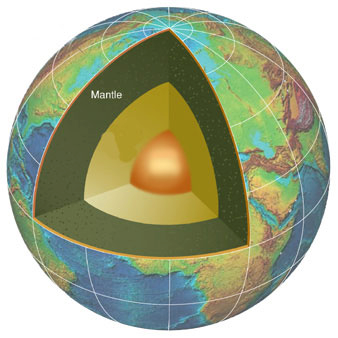
\includegraphics[width=0.8\textwidth]{earths-mantel.png}\\
\vspace{5mm}\hspace{47mm}\tiny{Image: mail.colonial.net}
\end{columns}
\end{frame}
%%
\begin{frame}\frametitle{Mantle Convection}
\begin{columns}
\hspace*{-8mm}
\column[T]{0.45\textwidth}
\vspace{6mm}
\begin{myColorBox}{.8}{}\color{linkcolor}
\centering
\begin{itemize}
 \item Global models became available in the late 80s
 \item They were parallelized in the 90s
\end{itemize}
\end{myColorBox}
\column[T]{0.55\textwidth}
\vspace{-5mm}
\begin{columns}
\column[T]{0.5\textwidth}
Glatzmeier, 1988\\
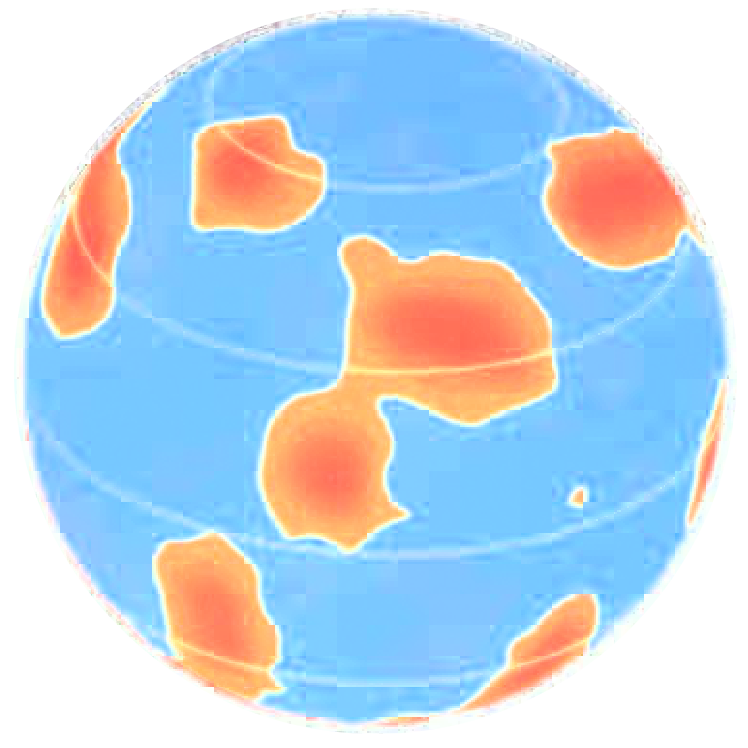
\includegraphics[width=0.9\textwidth]{glatzmeier88.png}\\
\vspace{2mm}
\hspace*{-4mm}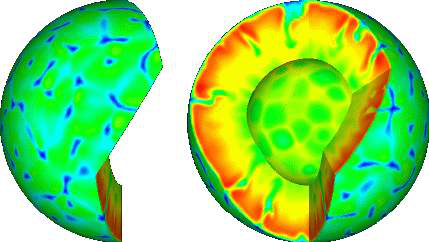
\includegraphics[width=1.1\textwidth]{bunge.png}\\
Bunge and Baumgardner, 1995
\column[T]{0.5\textwidth}
Baumgardner, 1985\\
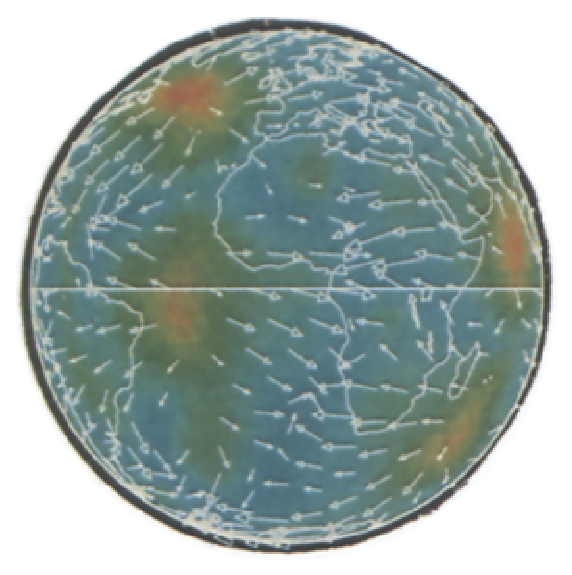
\includegraphics[width=0.9\textwidth]{baumgardner85.png}\\
\vspace{2mm}
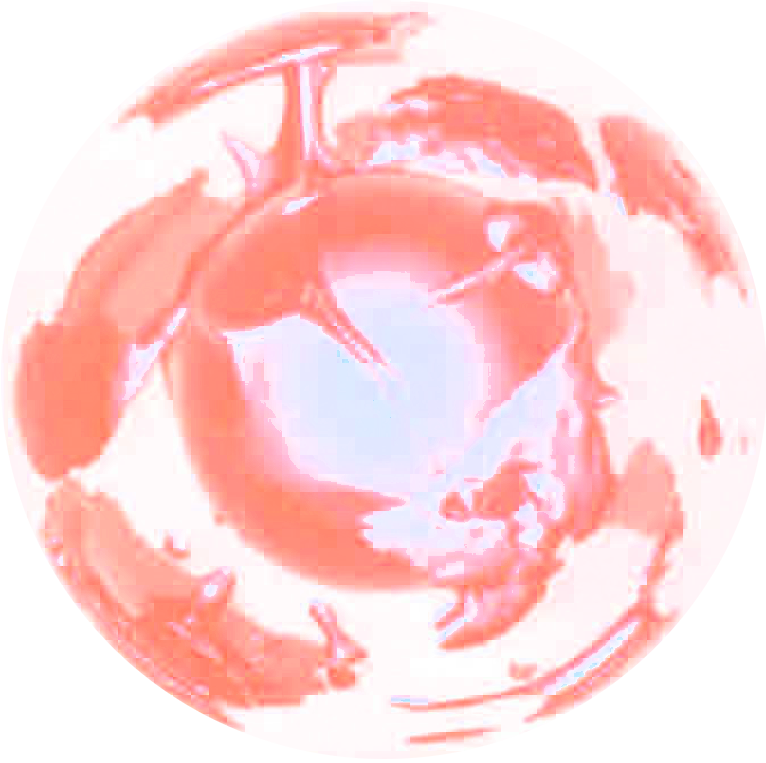
\includegraphics[width=0.9\textwidth]{tackley93.png}\\
Tackley et al, 1993
\end{columns}
\end{columns}
\end{frame}%%
\begin{frame}
\begin{columns}
\column[T]{0.55\textwidth}
\vspace{-6mm}
\begin{myColorBox}{.95}{}\color{linkcolor}
%\vspace*{-5mm}
\centering
%\hspace{-0mm}Thi (among others):
\begin{itemize}
 \item Convective planform (Earth and other planets)
 \item Link to seismology
 \item Geodetic observations
 \item Mineralogy
 \item Rheological effects
 \item Thermal evolution
 \item . . .
\end{itemize}
\end{myColorBox}
\vspace{-3mm}
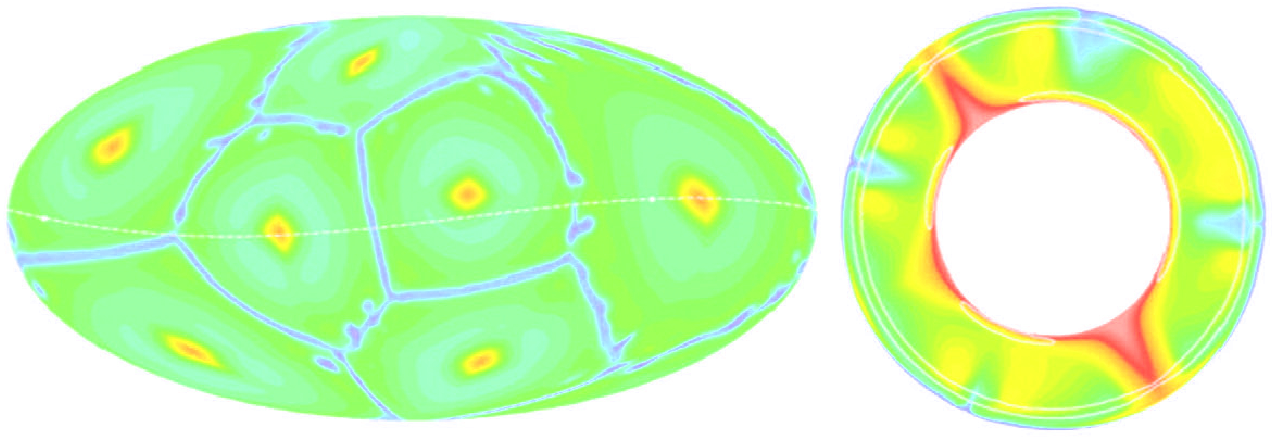
\includegraphics[width=1\textwidth]{tackley_12.png}\\ \scriptsize{Tackley, 2012}
\column[T]{0.45\textwidth}
\vspace{-4mm}
\scriptsize{Zhong et al, 2007}\\

\includegraphics[width=0.65\textwidth]{zhong_07.png}\\
\vspace{-6mm}
\flushright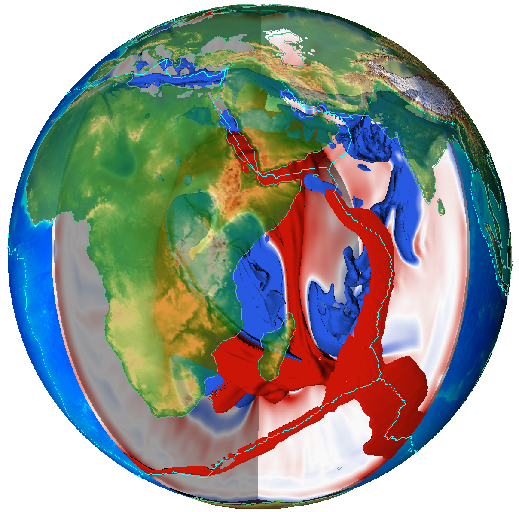
\includegraphics[width=0.65\textwidth]{MantlePicTerra.png}\\
\scriptsize{Schuberth et al, 2009}\\
\end{columns}
\end{frame}
%%
\begin{frame}\frametitle{Towards extreme resolutions}
\begin{columns}
\column[T]{0.55\textwidth}
\vspace*{5mm}
\begin{myColorBox}{.9}{}\color{linkcolor}
\centering
\begin{itemize}
 \item Most common codes scale to $\sim 1,000$ processors
 \item New class of problems:
 \begin{itemize}
  \item Fluid dynamic inverse models
  \item Complex non-linear problems
 \end{itemize}
 \item Current supercomputers have $\sim 1,000,000$ cores
\end{itemize}
\end{myColorBox}
\column[T]{0.45\textwidth}
\centering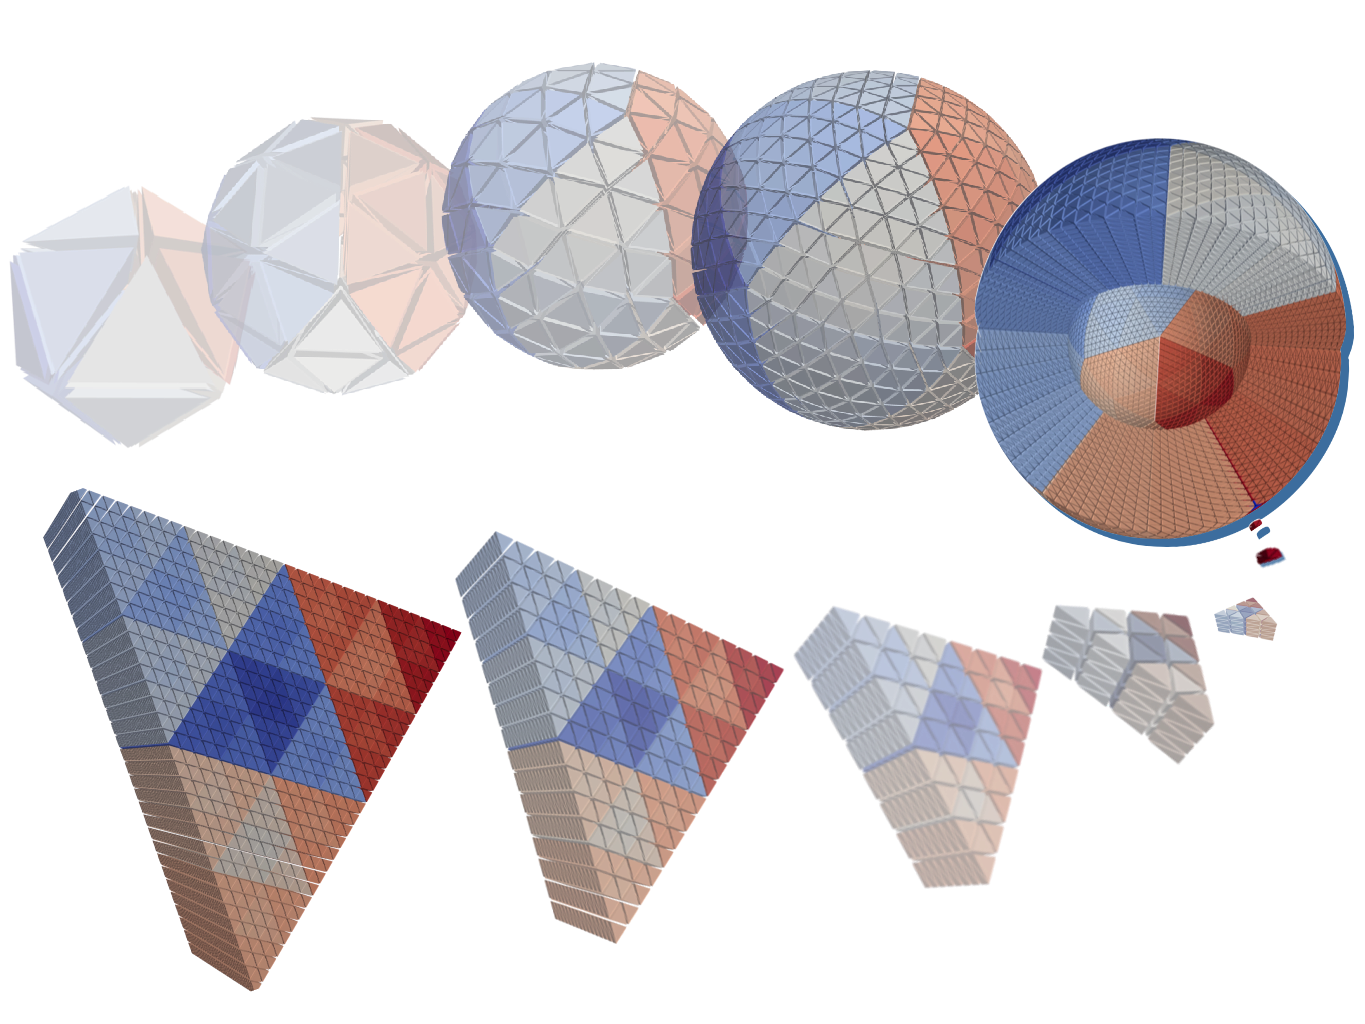
\includegraphics[width=\textwidth]{earth-collage.png}\\
\end{columns}
\end{frame}
%%
\begin{frame}\frametitle{Future Exascale Challenges}
\vspace*{-3mm}
\centering
\begin{myColorBox}{.7}{}\color{linkcolor}
\begin{itemize}
 \item Millions of processing units
 \item Heterogeneous hardware:
\begin{itemize}
 \item many-core
 \item accelerators
 \item GPUs
\end{itemize}
 \item Resilience
 \item . . .
\end{itemize}
\end{myColorBox}
\begin{itemize}
 \item Priority program by the German research funding agency
 \item Funding 13 application science projects
\end{itemize}
%\vspace{8mm}
\hspace{13mm}

\includegraphics[height=0.13\textheight]{sppexa.png}
\hspace{13mm}

\includegraphics[height=0.17\textheight]{tn-logo-crop.pdf}
\end{frame}
%%
\section{Equations}
\subsection*{Equations}
%%
\begin{frame}\frametitle{Governing equations}
\only<1>{
\vspace*{-3mm}
\begin{myColorBox}{.8}{}\color{linkcolor}
\vspace*{-5mm}
\centering
\begin{equation*}
\left.
\begin{align}
 \quad\quad{\eta \Delta \vec{u}} - \grad p + \mbox{Ra} T &= 0 \quad \\
 \div \vec{u} &= 0 \\
\end{align}
\right\} \,\, \mbox{Stokes equations}  \,
\end{equation*}
\begin{equation*}
\left. \dt T = - \vec{u} \cdot \grad{T} - \kappa\, \Delta T \quad\right \} \,\,\,\,\mbox{Heat equation}
\end{equation*}\\
\end{myColorBox}
\vspace*{2ex}
\begin{itemize}
 \item Simplified Navier-Stokes equations
 \item Slow deformation by creep
\end{itemize}
}
%%
\only<2>{
\vspace*{-3mm}
\begin{myColorBox}{.8}{}\color{linkcolor}
\vspace*{-5mm}
\centering
\begin{equation*}
\left.
\begin{align}
 \quad\quad{\color{blue}\eta \Delta \vec{u}} - \grad p + {\color{blue}\mbox{Ra} T} &= 0 \quad \\
 \div \vec{u} &= 0 \\
\end{align}
\right\} \,\, \mbox{Stokes equations}  \,
\end{equation*}
\begin{equation*}
\left. \dt T = - \vec{u} \cdot \grad{T} - \kappa\, \Delta T \quad\right \} \,\,\,\,\mbox{Heat equation}
\end{equation*}\\
\end{myColorBox}
\vspace*{2ex}
\begin{itemize}
 \item Simplified Navier-Stokes equations
 \item Slow deformation by creep
 \item {\color{blue}Force balance between friction and buoyancy}
\end{itemize}
}
%%
\only<3>{
\vspace*{-3mm}
\begin{myColorBox}{.8}{}\color{linkcolor}
\vspace*{-5mm}
\centering
\begin{equation*}
\left.
\begin{align}
 \quad\quad{\color{red}\eta \Delta \vec{u}} - \grad p + \mbox{Ra} T &= 0 \quad \\
 \div \vec{u} &= 0 \\
\end{align}
\right\} \,\, \mbox{Stokes equations}  \,
\end{equation*}
\begin{equation*}
\left. \dt T = - \vec{u} \cdot \grad{T} - \kappa\, \Delta T \quad\right \} \,\,\,\,\mbox{Heat equation}
\end{equation*}\\
\end{myColorBox}
\vspace*{2ex}
\begin{itemize}
 \item Simplified Navier-Stokes equations
 \item Slow deformation by creep
 \item Force balance between friction and buoyancy
 \item {\color{red}Dominated by viscous term ${\eta \Delta \vec{u}}$ \,\,$\Rightarrow$\,\, Global models}
\end{itemize}
}
%%
\only<4>{
\vspace*{-3mm}
\begin{myColorBox}{.8}{}\color{linkcolor}
\vspace*{-5mm}
\centering
\begin{equation*}
\left.
\begin{align}
 \quad\quad{\eta \Delta \vec{u}} - \grad p + \mbox{Ra} T &= 0 \quad \\
 \div \vec{u} &= 0 \\
\end{align}
\right\} \,\, \mbox{Stokes equations}  \,
\end{equation*}
\begin{equation*}
\left. {\color{blue}\dt T} = - \vec{u} \cdot \grad{T} - \kappa\, \Delta T \quad\right \} \,\,\,\,\mbox{Heat equation}
\end{equation*}\\
\end{myColorBox}
\vspace*{2ex}
\begin{itemize}
 \item Simplified Navier-Stokes equations
 \item Slow deformation by creep
 \item Force balance between friction and buoyancy
 \item Dominated by viscous term ${\eta \Delta \vec{u}}$ \,\,$\Rightarrow$\,\, Global models
 \item {\color{blue}Time derivative only in heat equation}
\end{itemize}
}
\end{frame}
%%
\begin{frame}\frametitle{Governing equations}
\only<1>{
\vspace*{-3mm}
\begin{myColorBox}{.8}{}\color{linkcolor}
\vspace*{-5mm}
\centering
\begin{equation*}
\left.
\begin{align}
 \quad\quad{\eta \Delta \vec{u}} - \grad p + \mbox{Ra} T &= 0 \quad \\
 \div \vec{u} &= 0 \\
\end{align}
\right\} \,\, \mbox{Stokes equations}  \,
\end{equation*}
\begin{equation*}
\left. \dt T = - \vec{u} \cdot \grad{T} - \kappa\, \Delta T \quad\right \} \,\,\,\,\mbox{Heat equation}
\end{equation*}\\
\end{myColorBox}
\vspace{3mm}
\hspace{15mm}
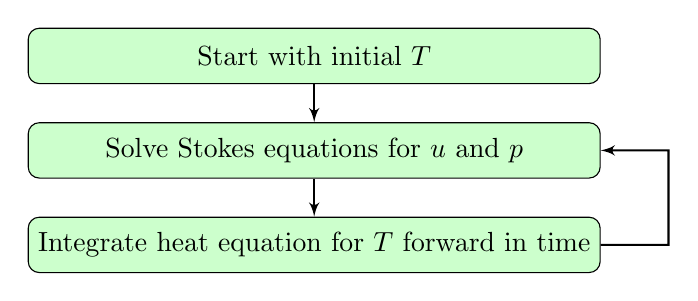
\begin{tikzpicture}[node distance = 12mm, auto]
  \node [block] (a) {Start with initial $T$};
  \node [block, below of=a] (b) {Solve Stokes equations for $\vec{u}$ and $p$};
  \node [block, below of=b] (c) {Integrate heat equation for $T$ forward in time};
  \path [line] (a) -- (b);
  \path [line] (b) -- (c);
  \path [line] (c) -- +(4.5,0) -- +(4.5,1.2) -- (b);
\end{tikzpicture}
}
%%
\only<2>{
\vspace*{-3mm}
\begin{myColorBox}{.8}{}\color{linkcolor}
\vspace*{-5mm}
\centering
\begin{equation*}
\left.
\begin{align}
\color{blue} \quad\quad{\eta \Delta \vec{u}} - \grad p + \mbox{Ra} T &\color{blue}= 0 \quad \\
\color{blue} \div \vec{u} &\color{blue}= 0 \\
\end{align}
\color{blue}\right\} \,\, \mbox{\color{blue}Stokes equations}  \,
\end{equation*}
\begin{equation*}
\left. \dt T = - \vec{u} \cdot \grad{T} - \kappa\, \Delta T \quad\right \} \,\,\,\,\mbox{Heat equation}
\end{equation*}\\
\end{myColorBox}
\vspace{3mm}
\hspace{15mm}
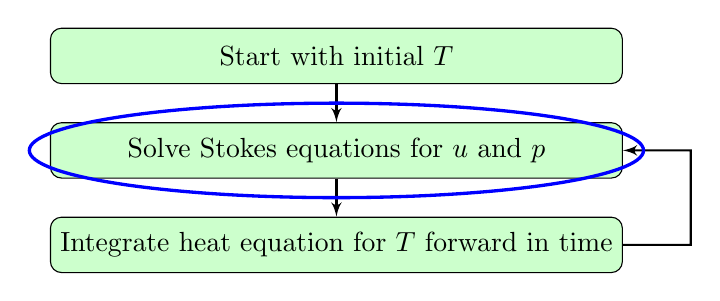
\begin{tikzpicture}[node distance = 12mm, auto]
  \node [block] (a) {Start with initial $T$};
  \node [block, below of=a] (b) {Solve Stokes equations for $\vec{u}$ and $p$};
  \node [block, below of=b] (c) {Integrate heat equation for $T$ forward in time};
  \path [line] (a) -- (b);
  \path [line] (b) -- (c);
  \path [line] (c) -- +(4.5,0) -- +(4.5,1.2) -- (b);
  \draw [blue,very thick] (0,-1.2) ellipse [ x radius=3.9, y radius=.6];
\end{tikzpicture}
}
\end{frame}
%%
\begin{frame}\frametitle{Solving the Stokes equations}
\vspace*{-3mm}
\begin{myColorBox}{.8}{}\color{linkcolor}
\vspace*{-5mm}
\centering
\begin{equation*}
\left.
\begin{align}
 \quad\quad{\eta \Delta \vec{u}} - \grad p + \mbox{Ra} T &= 0 \quad \\
 \div \vec{u} &= 0 \\
\end{align}
\right\} \,\, \mbox{Stokes equations}  \,
\end{equation*}
\begin{equation*}
\left. \dt T = - \vec{u} \cdot \grad{T} - \kappa\, \Delta T \quad\right \} \,\,\,\,\mbox{Heat equation}
\end{equation*}\\
\end{myColorBox}
%\vspace*{1.4ex}
\vspace*{-2mm}
\begin{itemize}
 \item So called saddle point problem:
\end{itemize}
\vspace*{-2mm}
\begin{myColorBox}{.8}{}\color{linkcolor}
\vspace*{-5mm}
\centering
\begin{equation*}
\left( \begin{array}{cc}
\mathbf{A} & \mathbf{B}^{\mbox{\tiny{T}}} \\
\mathbf{B} & \mathbf{0} \\
\end{array}\right)
\left( \begin{array}{c}
\mathbf{u} \\
\mathbf{p} \\
\end{array}\right) =
\left( \begin{array}{c}
\mathbf{f} \\
\mathbf{0} \\
\end{array}\right)
\end{equation*}
\end{myColorBox}
\vspace*{-2mm}
\begin{itemize}
 \item Many different solution schemes
 \item All need solution of Poisson equation
 \item Multigrid
\end{itemize}
\end{frame}
%%

% =============================================================================
%    Results for spherepoisson
% =============================================================================
%
% =============================================================================
%
\begin{frame}\frametitle{Model problem}
We consider the PDE 
\begin{align*}
\div u &= f\quad \text{in }\Omega \\
     u &= 0\quad \text{on }\partial\Omega
\end{align*}
where $\Omega$ is a spherical shell
\begin{equation*}
\Omega = \left\{(x,y,z) \in\RR^3\quad:\quad 0.546^2 \leq x^2+y^2+z^2 \leq 1\right\}
\end{equation*}
and the right-hand side $f$ is given by
\begin{equation*}
f(x,y,z) = 3\cdot \sin(x)\sin(y)\sin(z).
\end{equation*}
%
\end{frame}
%
% =============================================================================
%
%
\section{Discretization}
\subsection{Discretization}
%
\begin{frame}\frametitle{Discretization}
In the classical HHG approach the spherical shell is approximated
by (at least 60) Tetrahedra (Macro-Tetrahedra).
This input grid is split into primitives of different dimensions 
(Vertices, Edges, Faces and \cempha{Tetrahedra})

\begin{figure}\centering
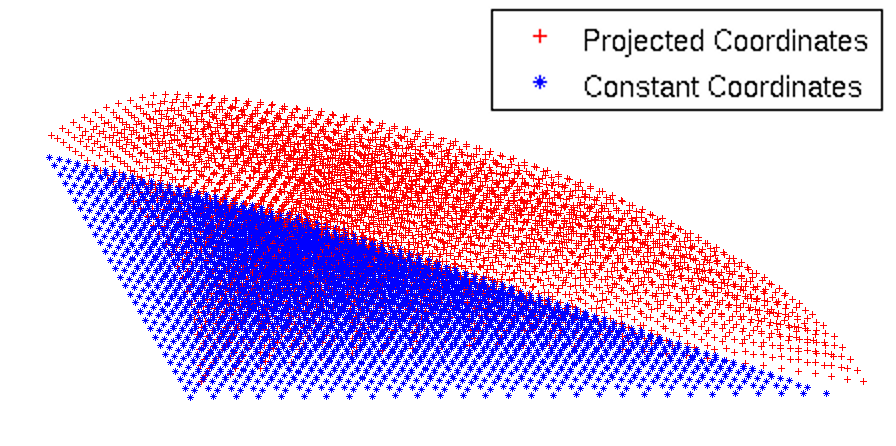
\includegraphics[width=0.5\textwidth]{macroTet_projected_constant_coords.png}
\caption{Inner nodes of one Macro Tetrahedron for refinement level 5. 
(Blue) classical (constant) coordinates in HHG 
(Red) Projected coordinates
}
\end{figure}



\end{frame}
%
% =============================================================================
%
\begin{frame}\frametitle{Major Problem with projected coordinates}
By projecting the coordinates onto the sphere, the fine grid tetrahedra
do not have the same volume any more, i.e we lose one of HHGs major advantages
(use the same local stiffness matrix for all refined nodes within one 
macro element)

As a consequence, we have to explicitly compute the local stiffness matrices
for each fine grid node on-the-fly, which 
   
   das gefaellt mir noch gar nicht !!



\end{frame}
%
% =============================================================================
%
\begin{frame}\frametitle{Const. vs. Projected Coordinates - Stencils}

\begin{columns}[T] 
\begin{column}[T]{4.1cm} 
  \centering
  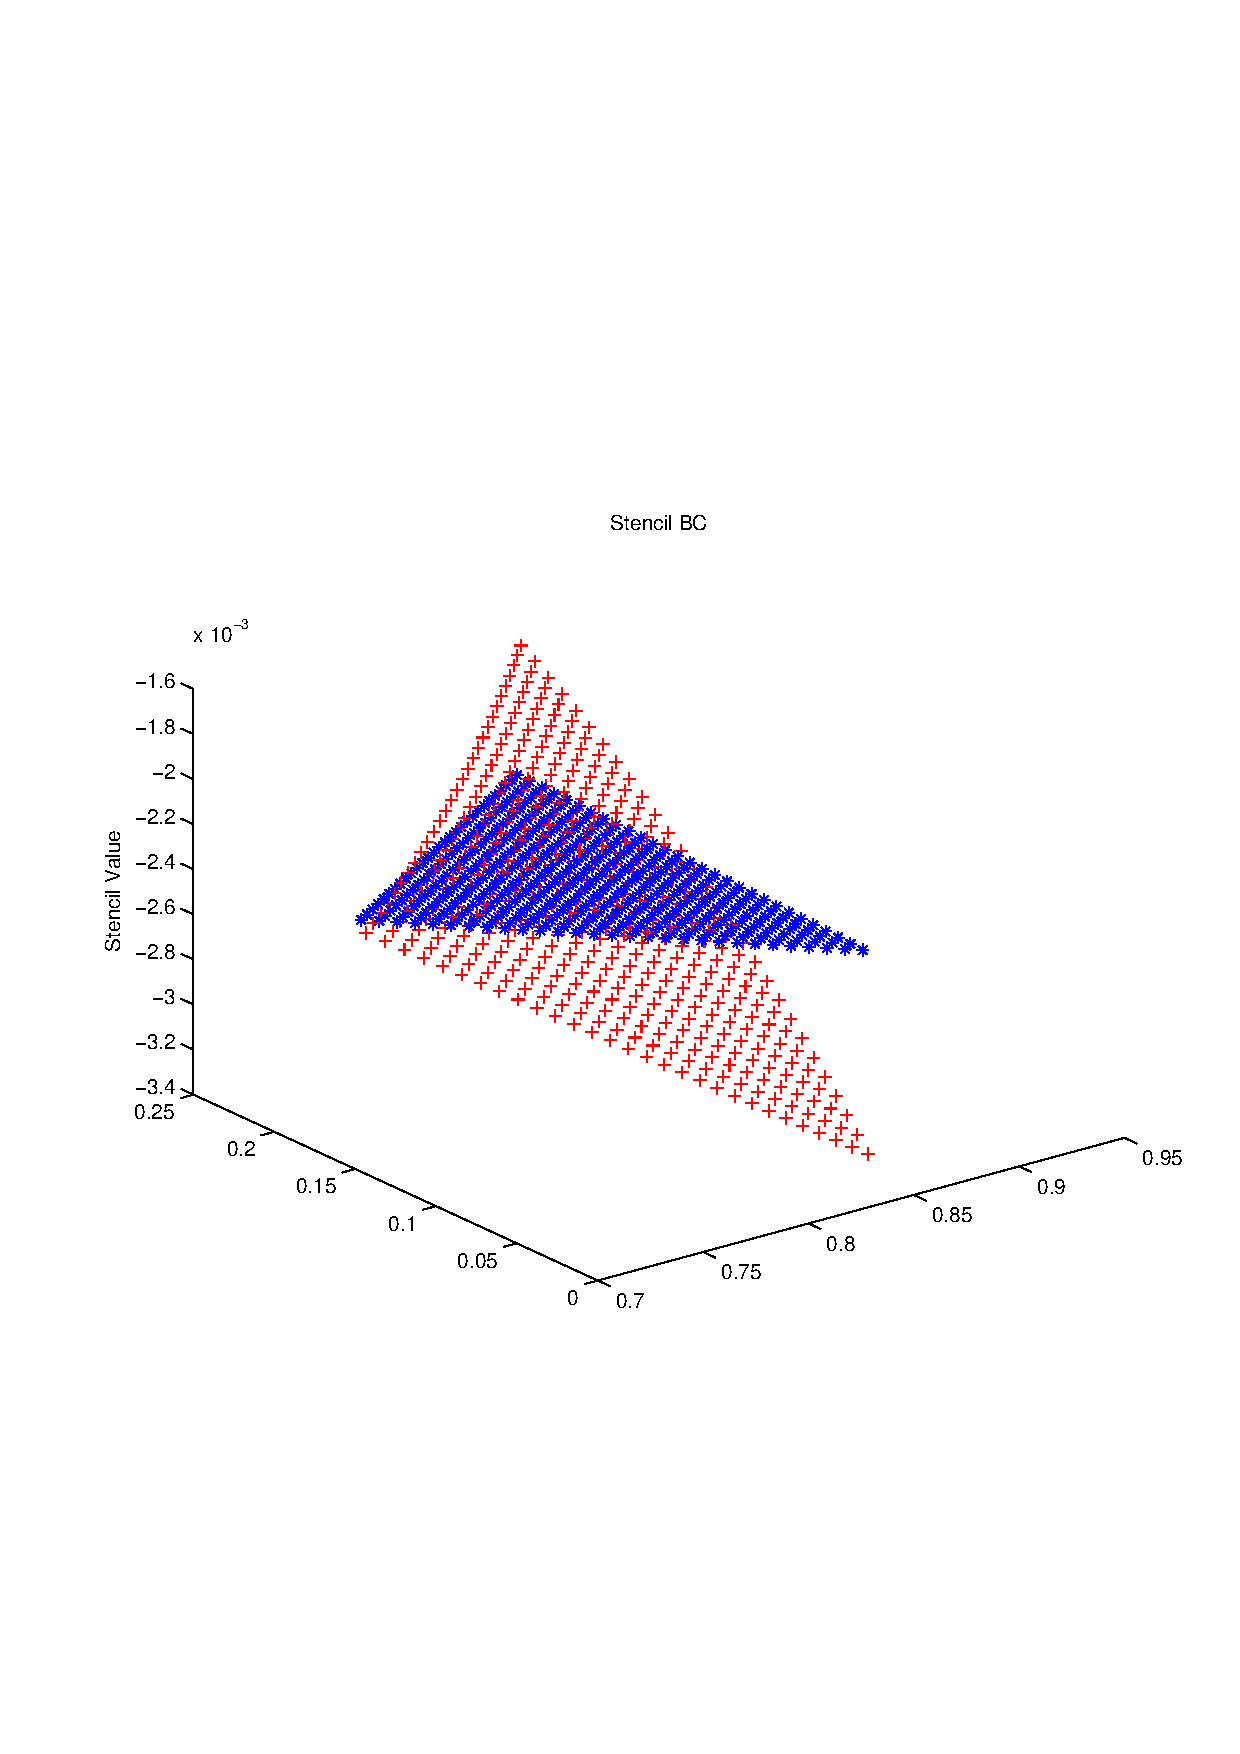
\includegraphics[width=0.98\textwidth]{stencilBC_nE}\\
  Stencil Entry BC
\end{column}\hfill
\begin{column}[T]{4.1cm} 
  \centering
  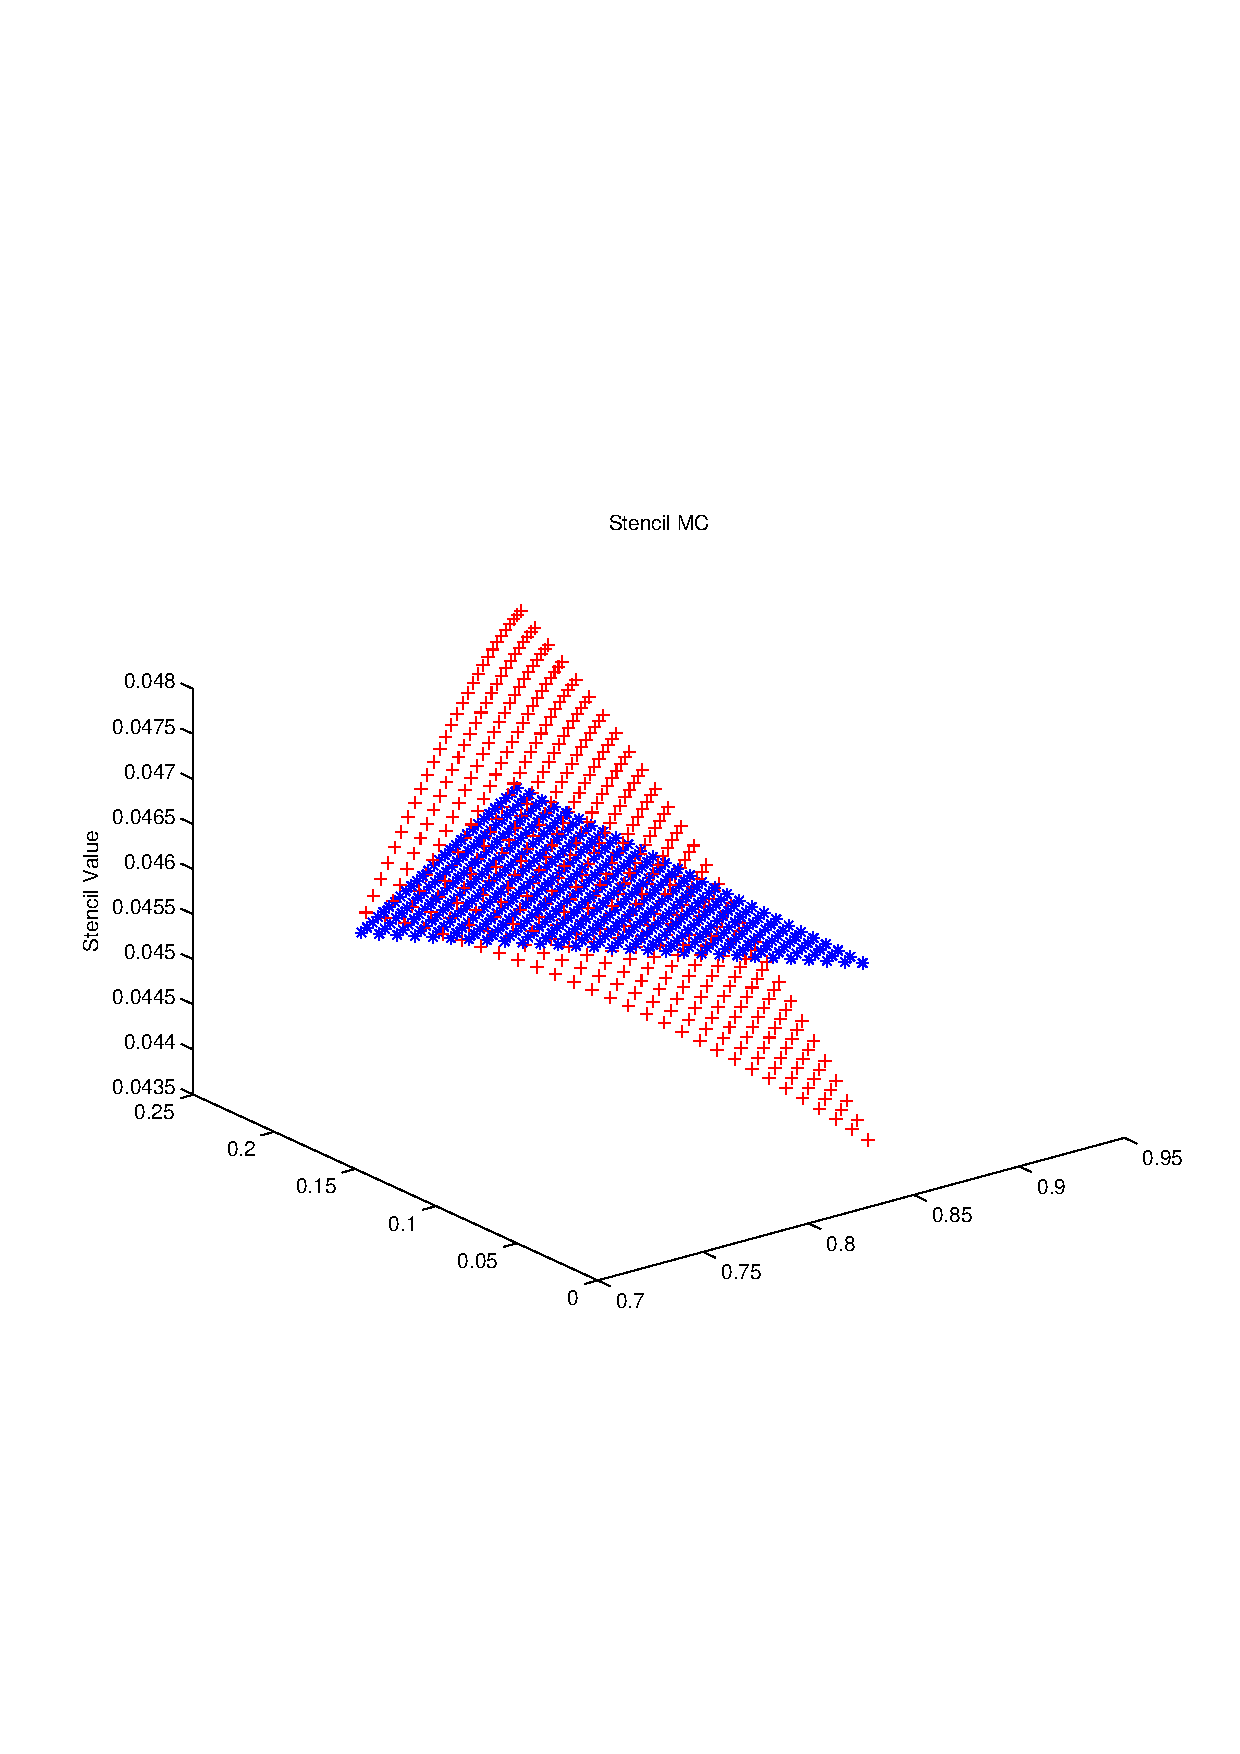
\includegraphics[width=0.98\textwidth]{stencilMC_nE}\\
  Stencil Entry MC
\end{column}\hfill
\begin{column}[T]{4.1cm} 
  \centering
  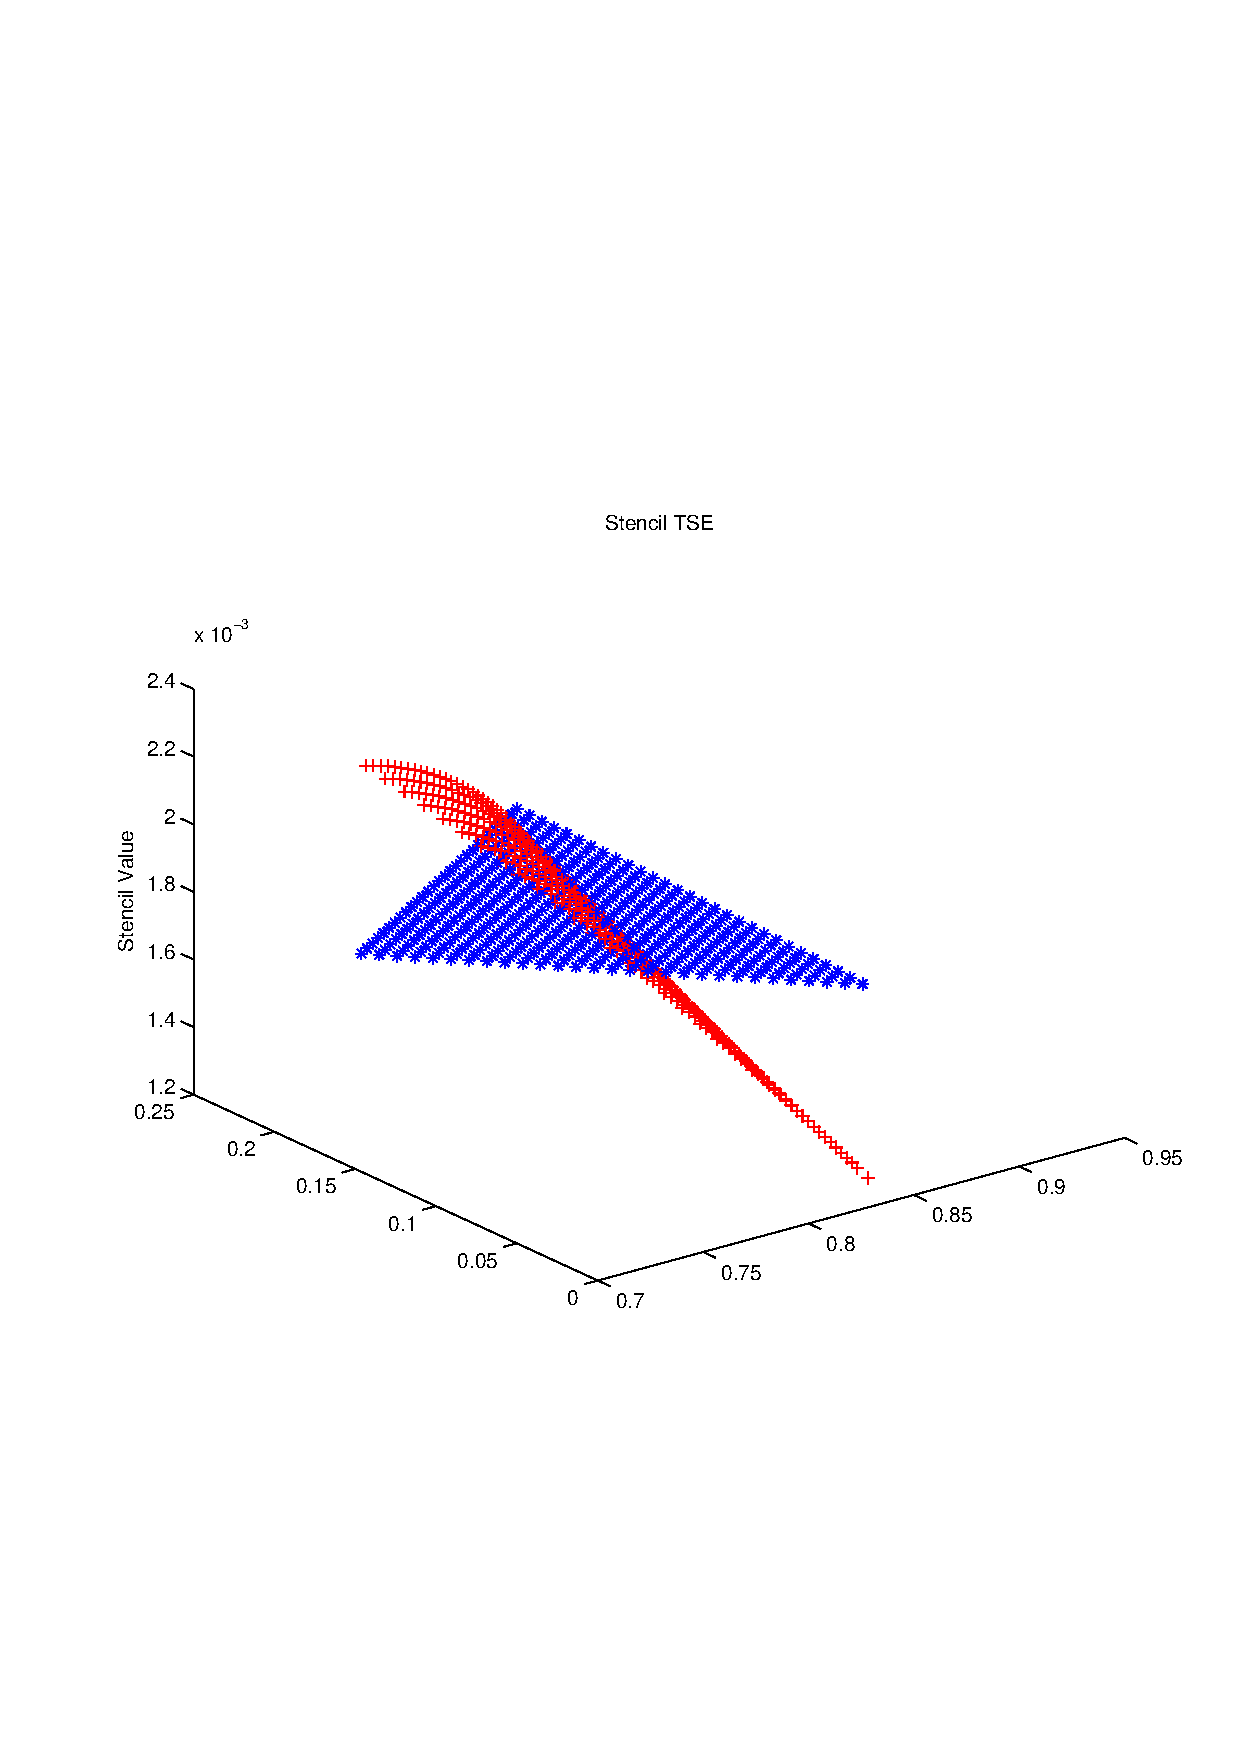
\includegraphics[width=0.98\textwidth]{stencilTSE_nE}\\
  Stencil Entry TSE
\end{column}
\end{columns}
\vspace{0.5cm}
\centering
Constant (blue) and projecte% =============================================================================
%    Results for spherepoisson
% =============================================================================
%
\section{Spherepoisson}
\subsection{Spherepoisson}d (red) stencil entries for all nodes of one plane
within one macro tetrahedron at refinement level 5


\end{frame}

%
% =============================================================================
%
\begin{frame}\frametitle{Stencils - Interpolation}


\rBox{Observation:} The displacements of the projected stencils exhibt
a smooth shape with some curvature.\\
\vspace{4ex}
\yBox{How can we utilize this?}\\
\vspace{4ex} 
\oBox{Idea:} Explicitly compute stencils only at some predefined sample
points and perform interpolation for all other points 

Questions: 
\begin{itemize}
\item{Which polynomial degree?}
\item{How much speed up can we gain?}
\item{Is this modified system still consistent with the original problem? }
\end{itemize}



\end{frame}

%
% =============================================================================
%
\begin{frame}\frametitle{Stencils - Interpolation }

\begin{itemize}
\item{linear    $\rightarrow$ not suitable due to the curvature}
\item{\oBox{quadratic} $\rightarrow$ resolves (moderate) curvature}
\item{cubic     $\rightarrow$ resolves curvature, but gets expensive}
\end{itemize}

\begin{figure}[htbp]
  \begin{minipage}{0.48\textwidth}   
For (tri-)quadratic interpolation we need 10 sample points.
This leads to the ansatz function:  
\begin{align*}
\label{eq:quadraticPolynomial}
a_{200}x^2 &+ a_{020}y^2 + a_{002}z^2 \\
+ a_{110}xy &+ a_{101}xz + a_{011}yz \\
+ a_{100}x &+ a_{010}y + a_{001}z \\
+ a_{000}
\end{align*}

  \end{minipage}
  \hfill
  \begin{minipage}{0.48\textwidth}
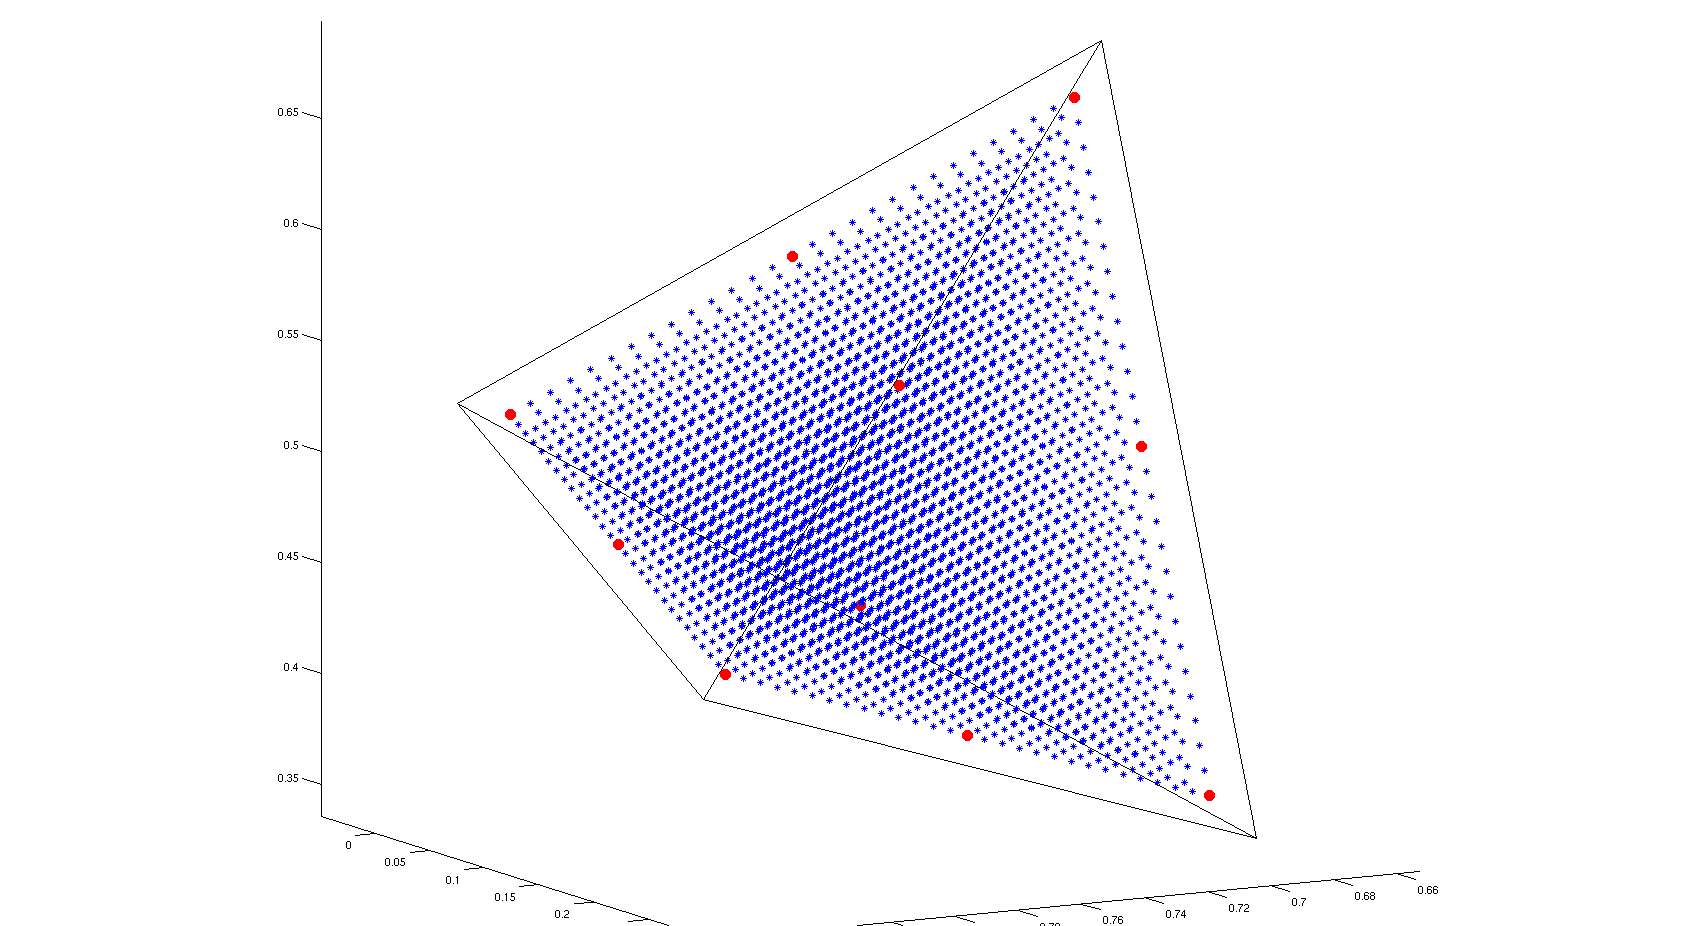
\includegraphics[width=0.98\textwidth]{tetSamplePointsPNG.png}
  \end{minipage}
\end{figure}


\end{frame}

%
% =============================================================================
%
\begin{frame}\frametitle{Interpolation - a first check}

\begin{columns}[T] 
\begin{column}[T]{4.1cm} 
  \centering
  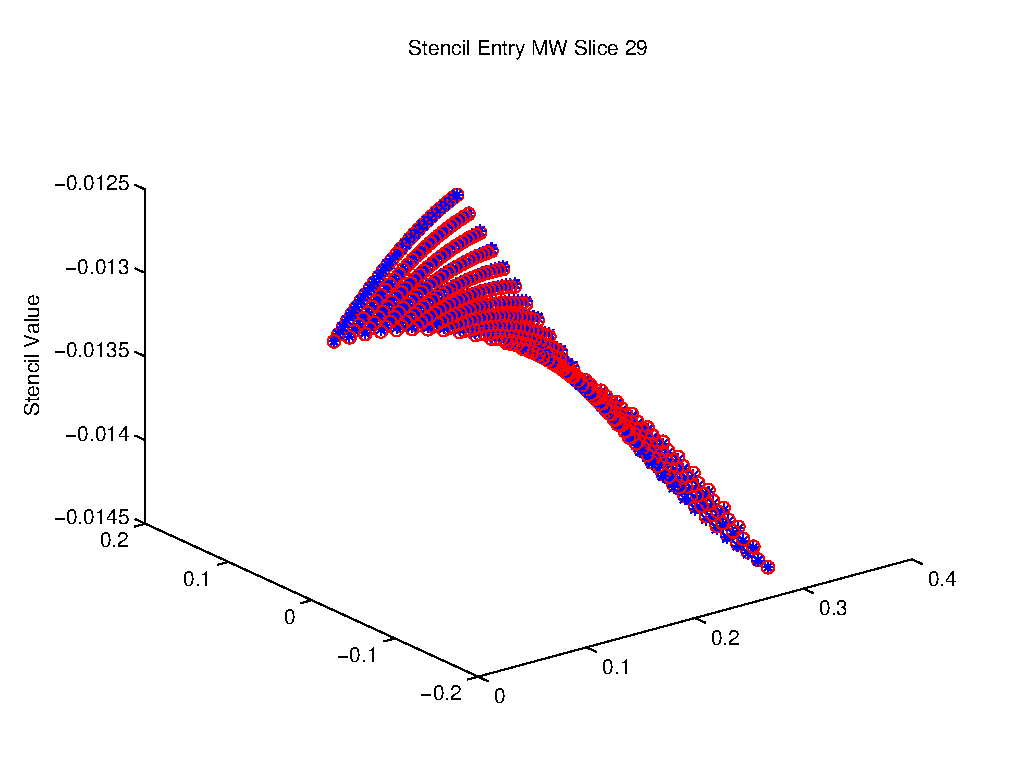
\includegraphics[width=0.98\textwidth]{stencilMW_slice29}\\
\end{column}\hfill
\begin{column}[T]{4.1cm} 
  \centering
  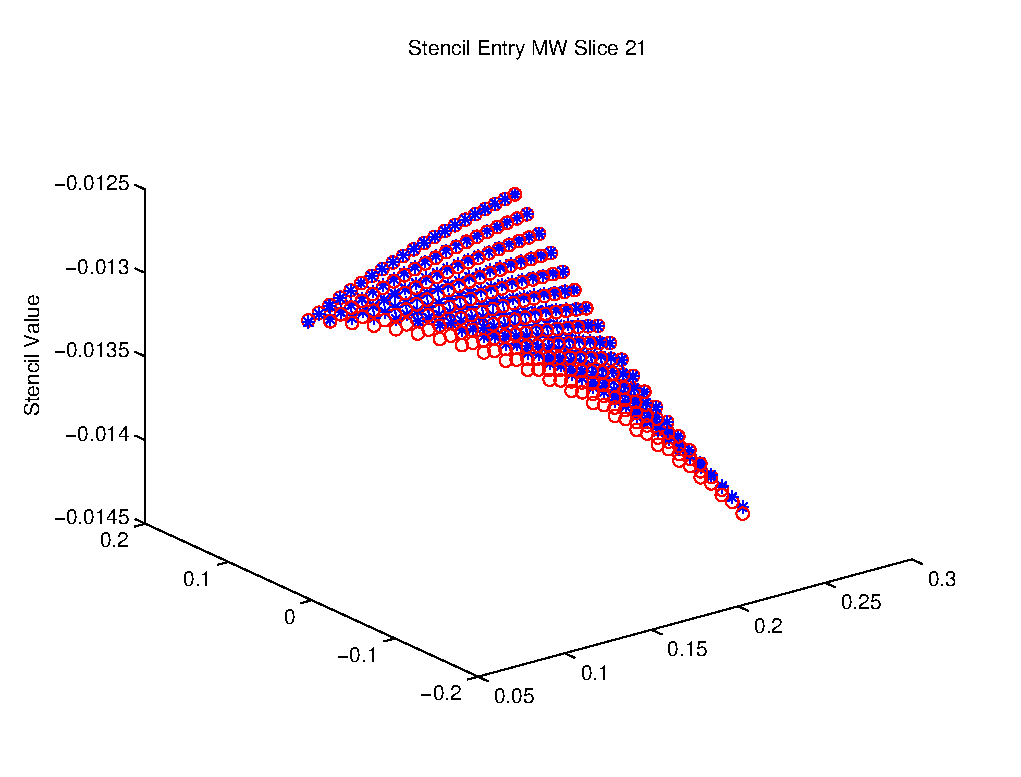
\includegraphics[width=0.98\textwidth]{stencilMW_slice21}\\
\end{column}\hfill
\begin{column}[T]{4.1cm} 
  \centering
  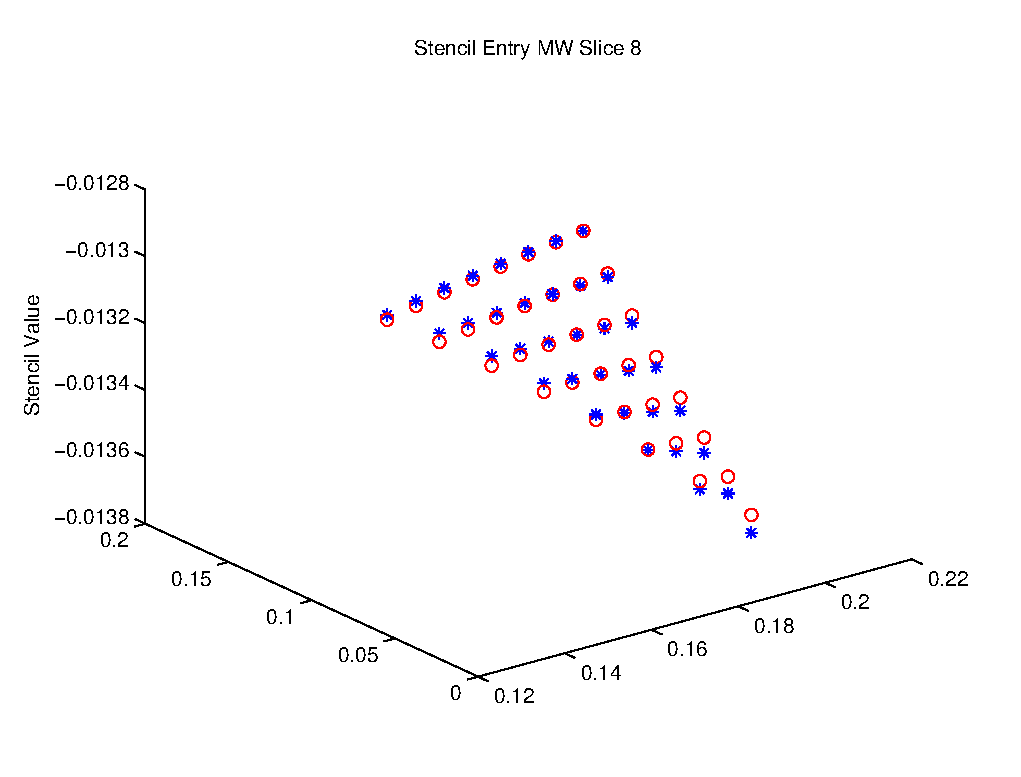
\includegraphics[width=0.98\textwidth]{stencilMW_slice8}\\
\end{column}
\end{columns}
\vspace{0.5cm}
\centering
Explicitly computed (projected) (blue dots) and interpolated 
(red circles) values for stencil entry
MW for different slices/planes within the macro tetrahedron
\end{frame}

%
% =============================================================================
%
\begin{frame}\frametitle{Interpolation of local stiffness matrices}


todo ...

\end{frame}

%
% =============================================================================
%
\begin{frame}\frametitle{Interpolation of local stiffness matrices}


\begin{theorem}
Both approaches are equivalent.
\end{theorem}

\begin{proof}
Schematically:\\
Employ the fact, that the functional
$\P_i : \RR^{10} \rightarrow \Pi^2$ which maps a
10-dimensional sample tuple 
onto a quadratic polynomial is \cempha{linear}.
Then, the order of stencil setup and interpolation 
can be reversed.
\end{proof}


\end{frame}

%
%
% =============================================================================
%
\begin{frame}\frametitle{HHG results - residual norm}

\begin{columns}[T] 
\begin{column}[T]{4.3cm} 
  \centering
  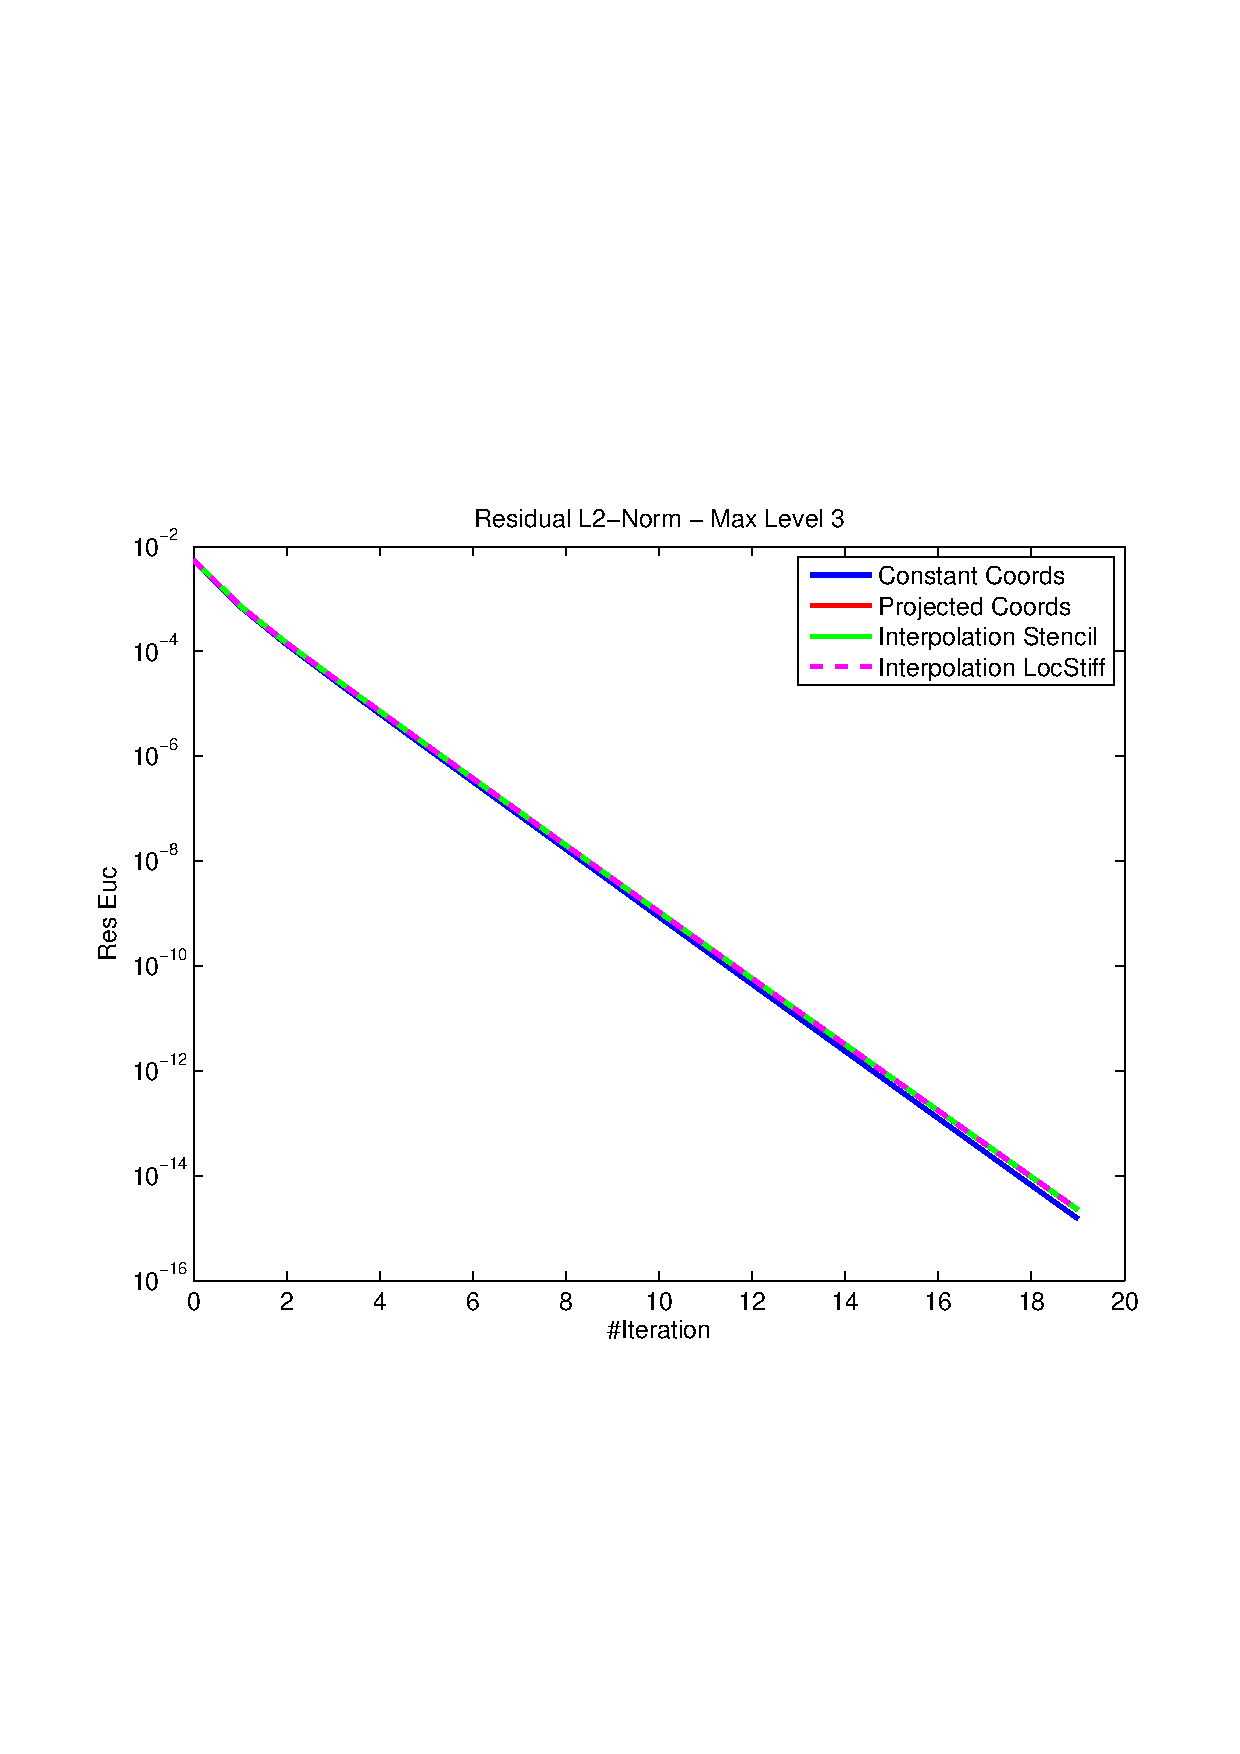
\includegraphics[width=0.98\textwidth]{spherepoisson_resEuc_level3}\\
  max. level 3
\end{column}\hfill
\begin{column}[T]{4.3cm} 
  \centering
  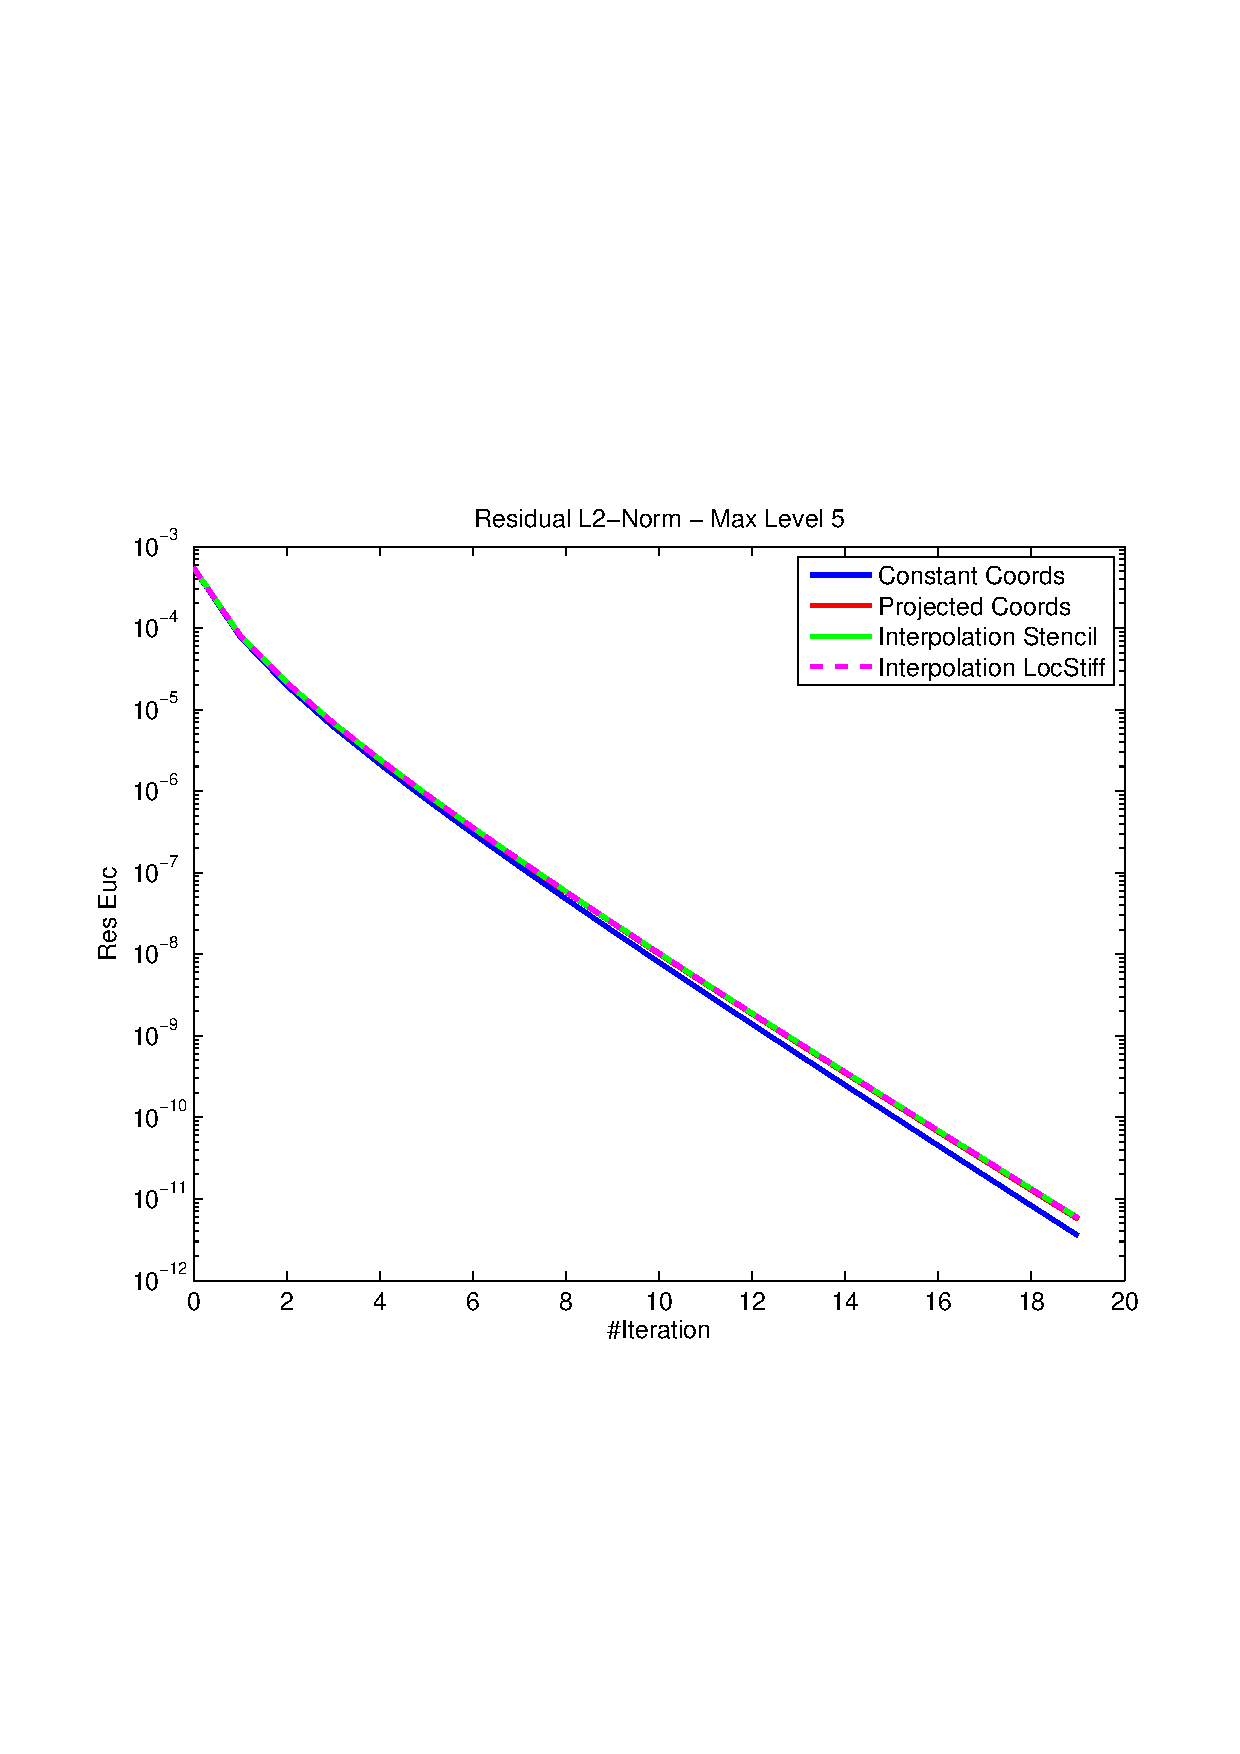
\includegraphics[width=0.98\textwidth]{spherepoisson_resEuc_level5}\\
  max. level 5
\end{column}\hfill
\begin{column}[T]{4.3cm} 
  \centering
  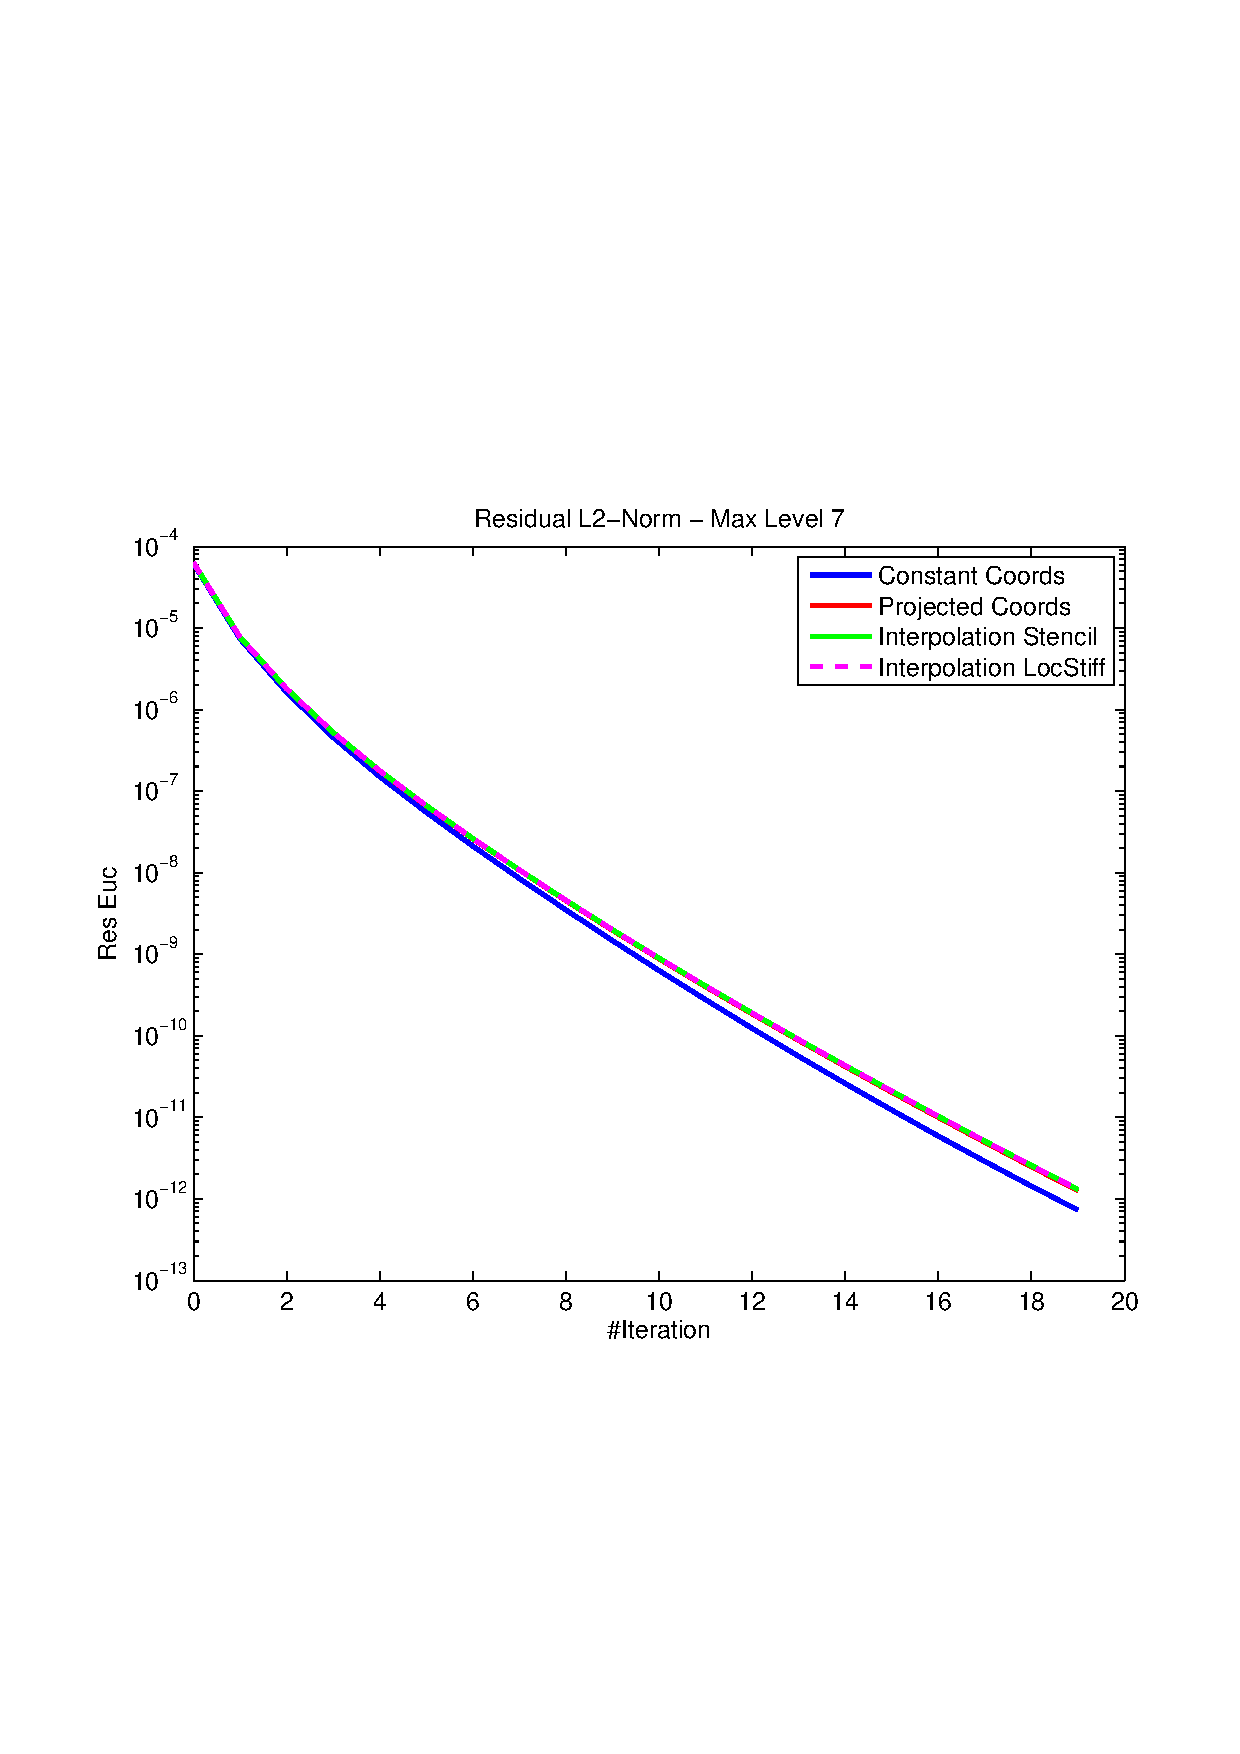
\includegraphics[width=0.98\textwidth]{spherepoisson_resEuc_level7}\\
  max. level 7
\end{column}
\end{columns}
\vspace{0.5cm}
\centering
Comparison of residual for constant (blue), projected (red), interpolated
stencil (green) and interpolated local stiffness matrices (magenta)
\end{frame}
%
%
% =============================================================================
%
\begin{frame}\frametitle{HHG results - CPU time}

\begin{columns}[T] 
\begin{column}[T]{4.3cm} 
  \centering
  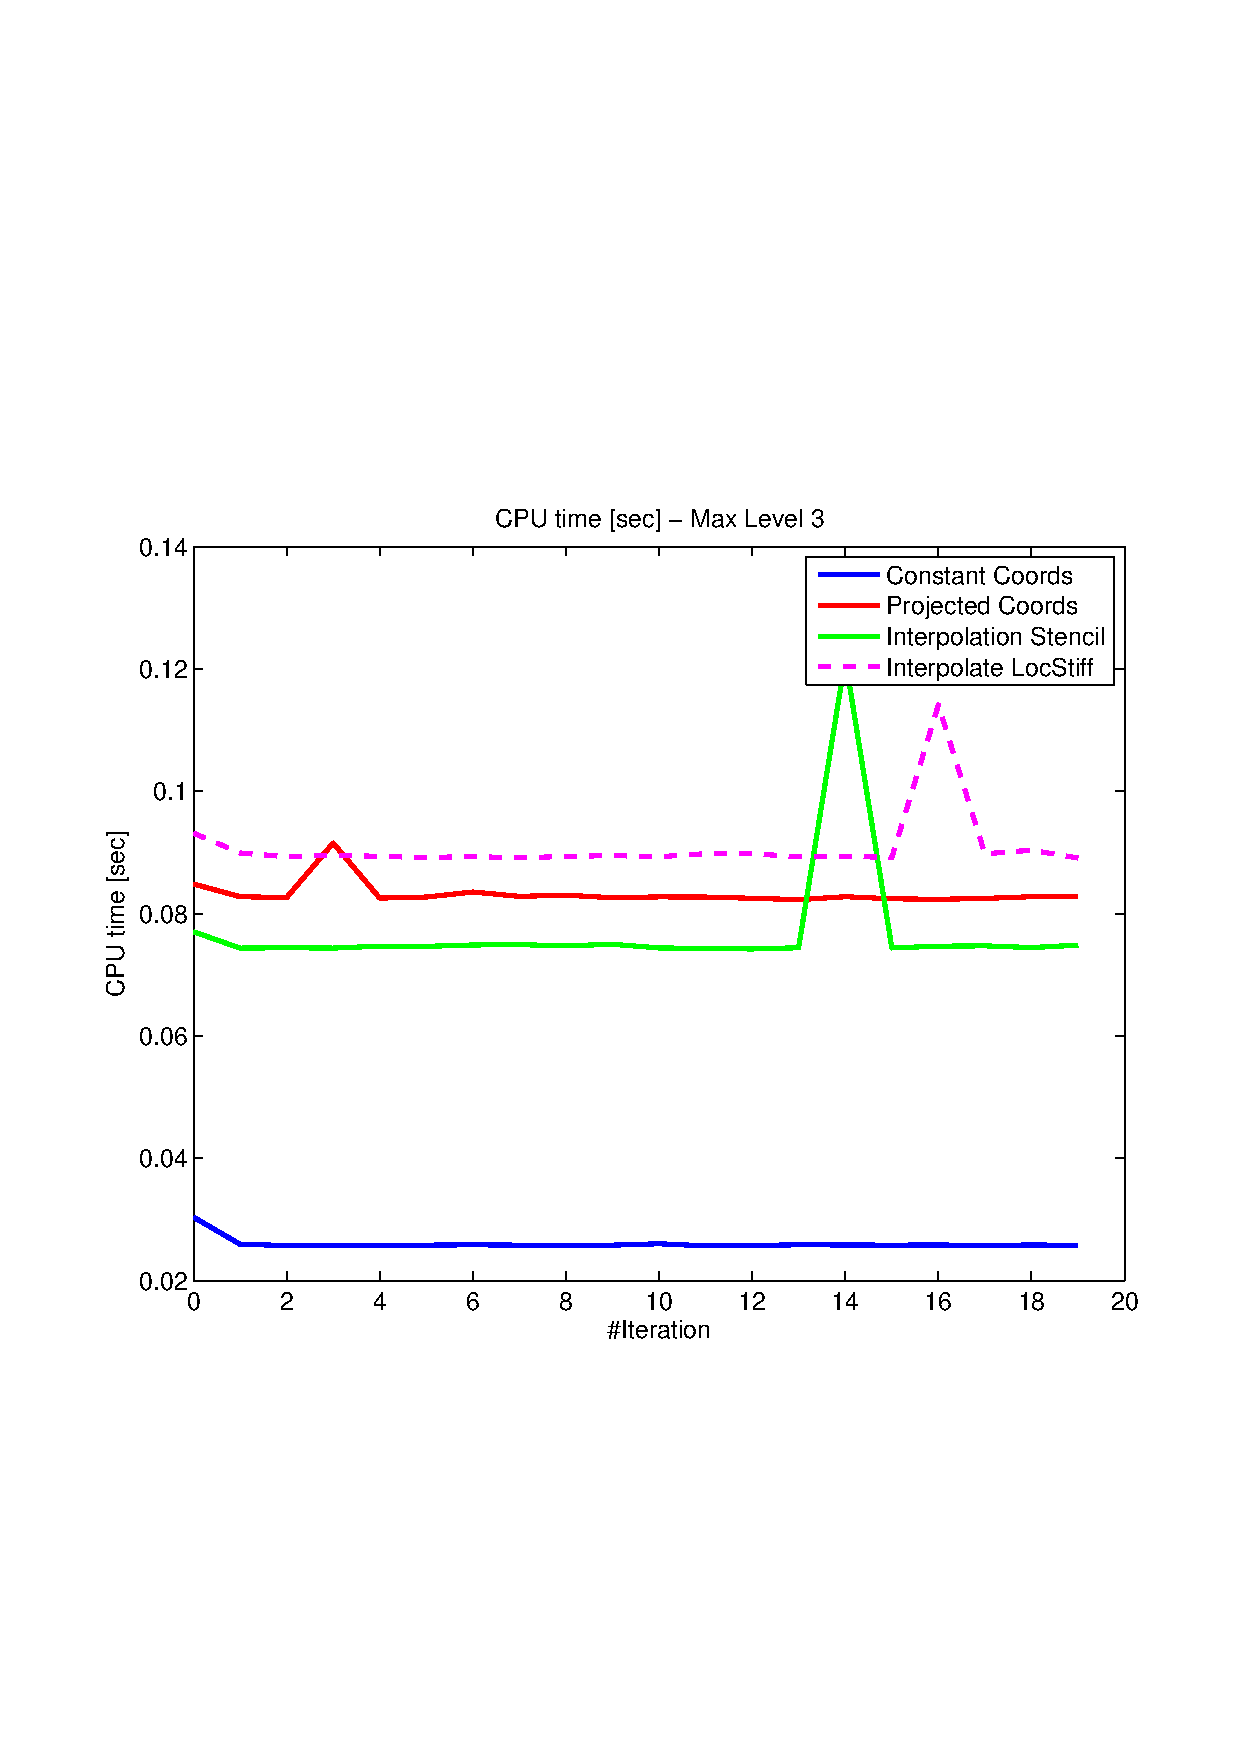
\includegraphics[width=0.98\textwidth]{spherepoisson_cpuTime_level3}\\
  max. level 3
\end{column}\hfill
\begin{column}[T]{4.3cm} 
  \centering
  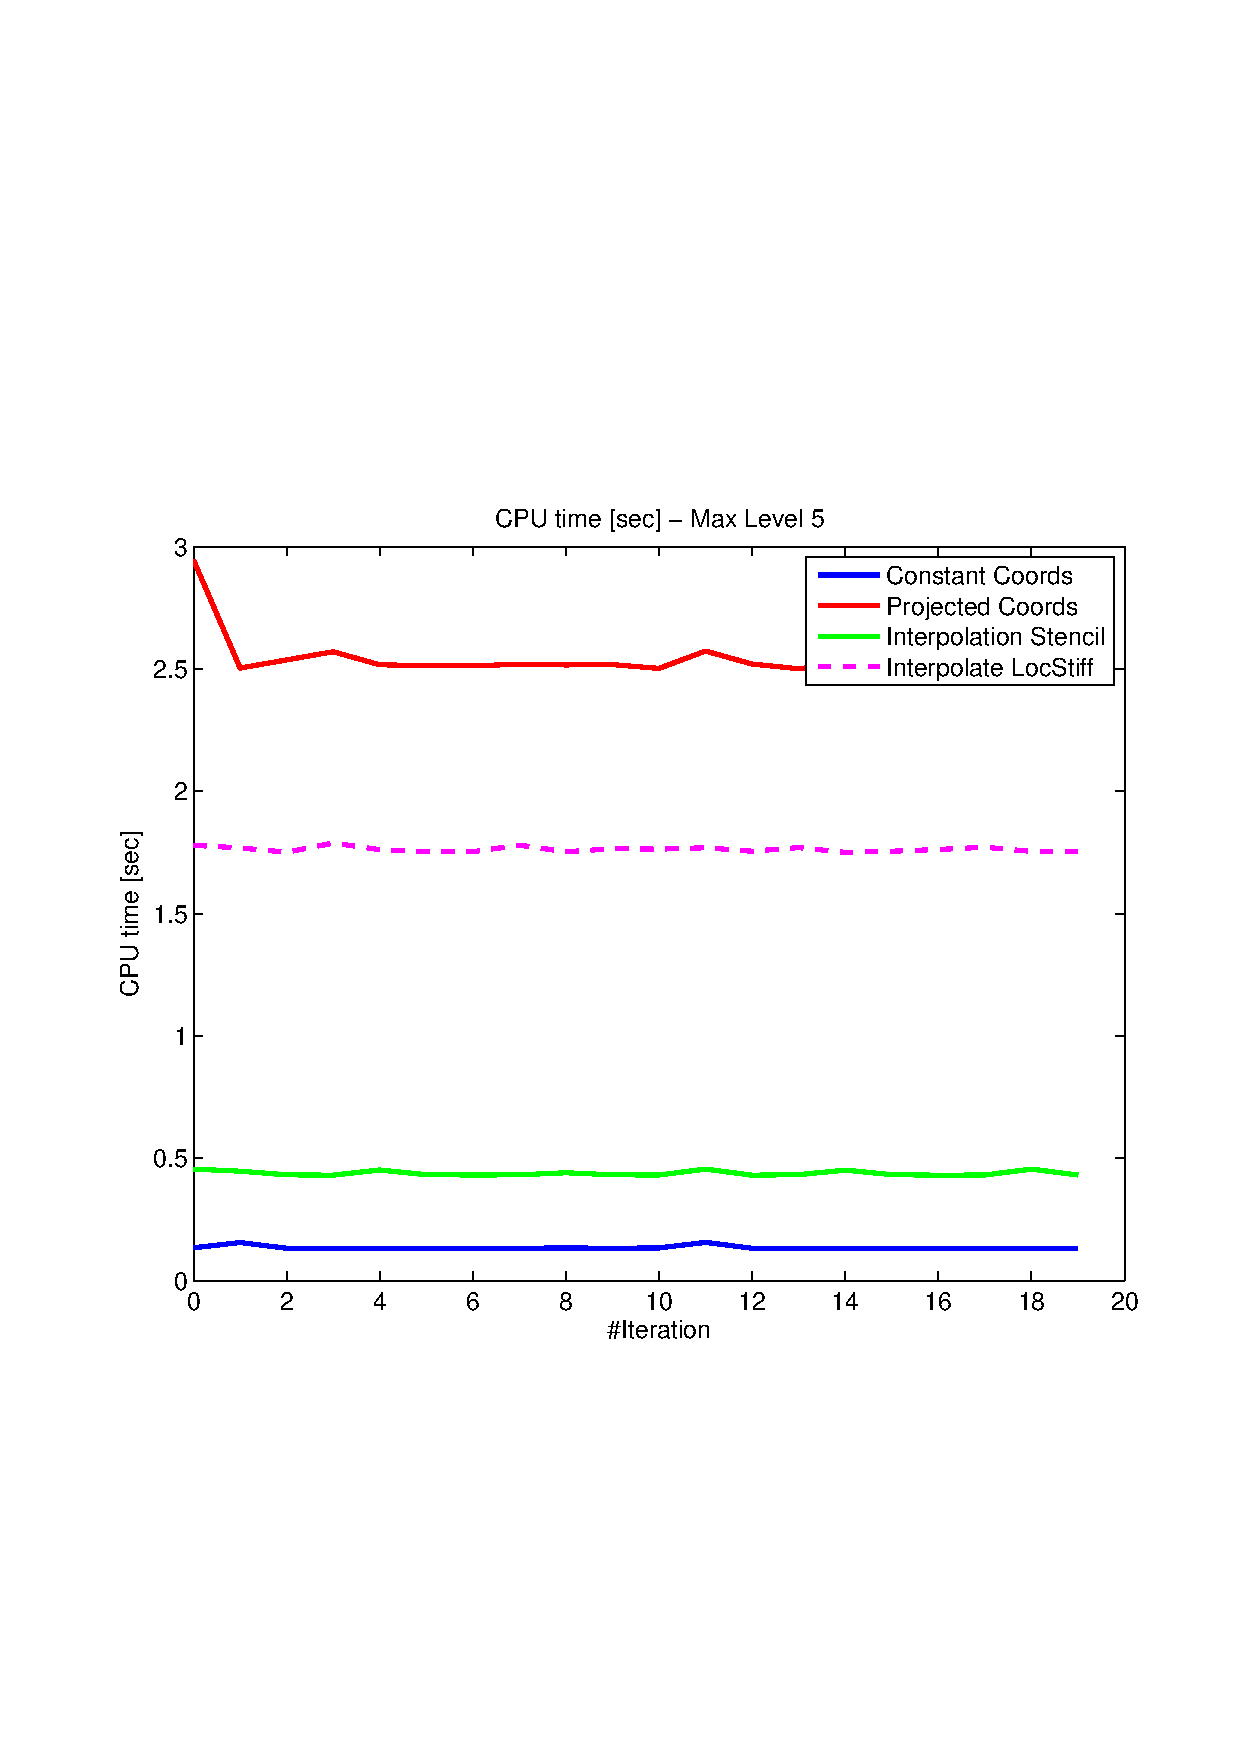
\includegraphics[width=0.98\textwidth]{spherepoisson_cpuTime_level5}\\
  max. level 5
\end{column}\hfill
\begin{column}[T]{4.3cm} 
  \centering
  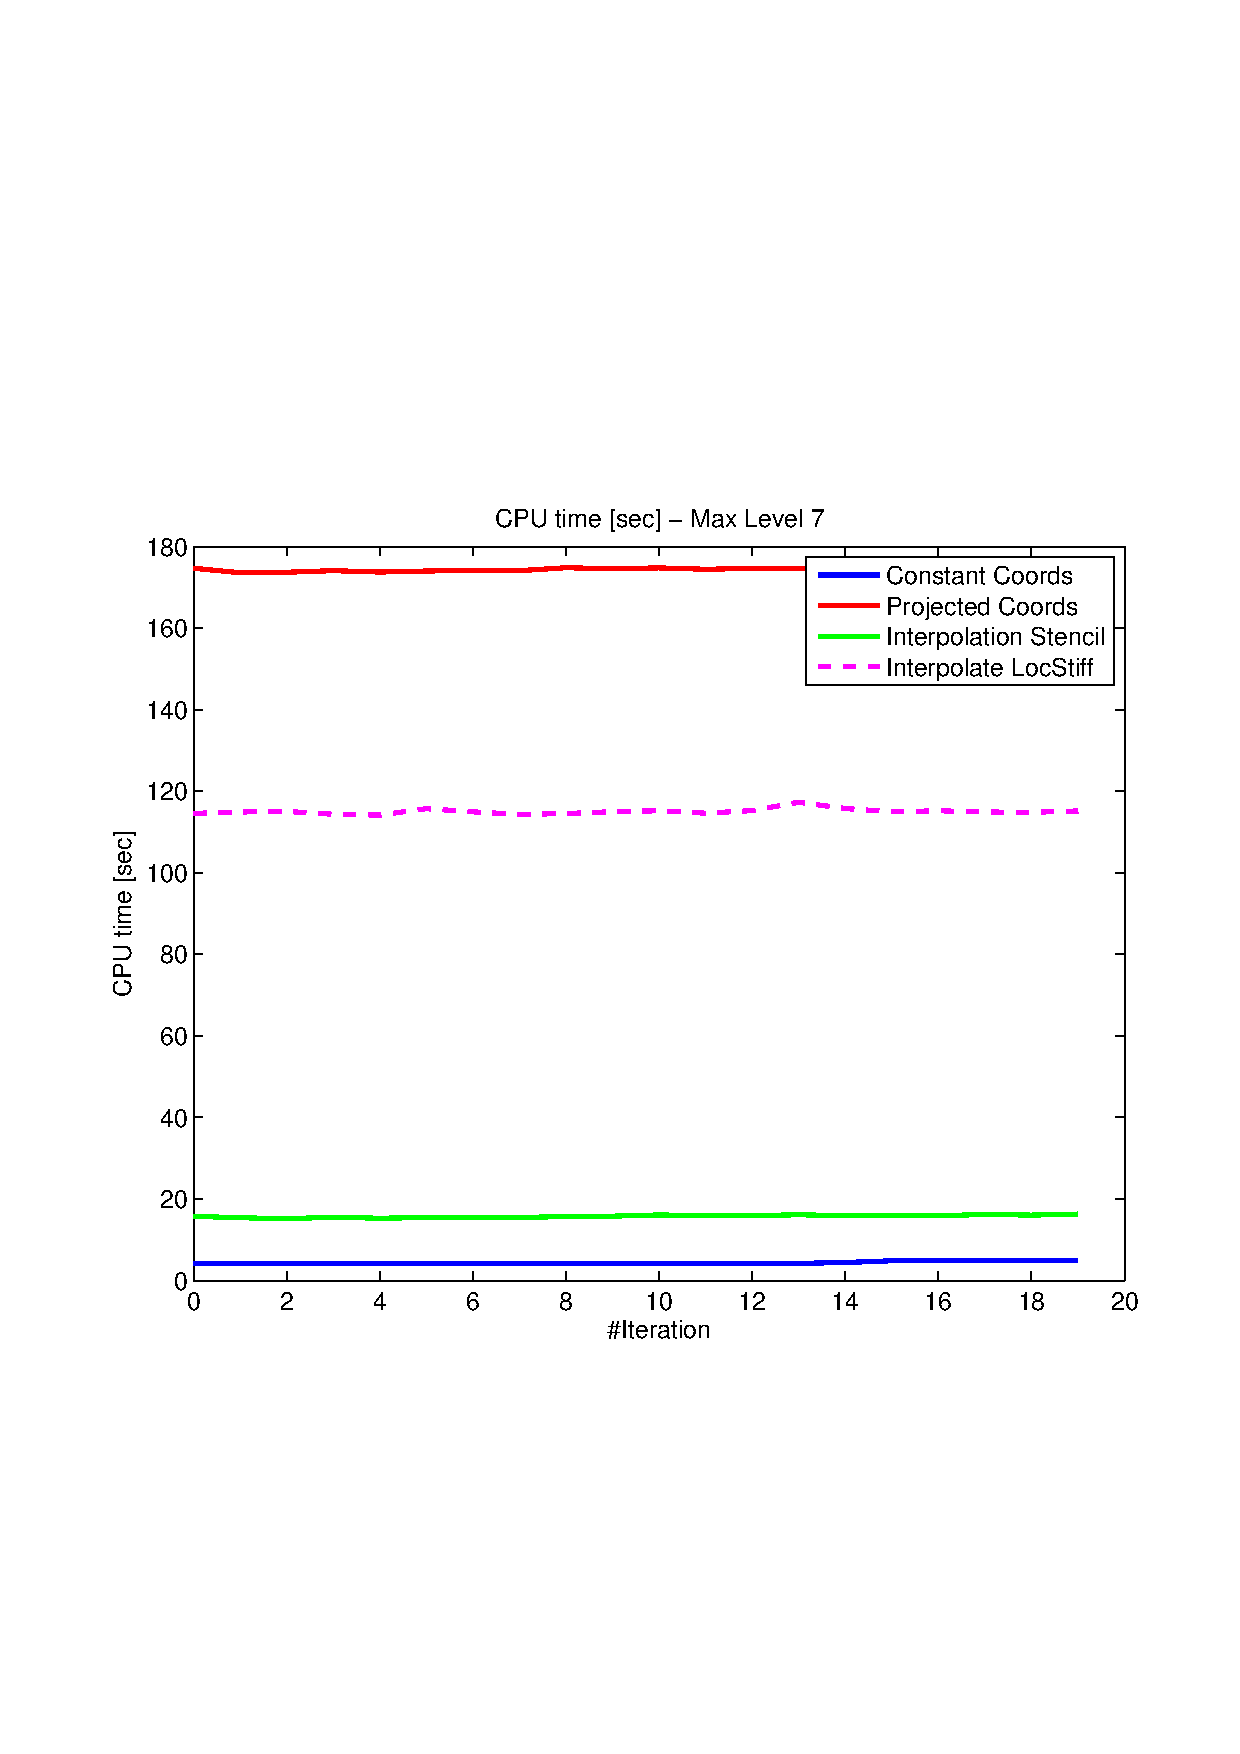
\includegraphics[width=0.98\textwidth]{spherepoisson_cpuTime_level7}\\
  max. level 7
\end{column}
\end{columns}
\vspace{0.5cm}
\centering
Comparison of CPU time [sec] for constant (blue), projected (red), interpolated
stencil (green) and interpolated local stiffness matrices (magenta).
Jobs were done on borgcube with 32 procs.
\end{frame}

%
% =============================================================================
%
\begin{frame}\frametitle{HHG results - Discretization error}

\begin{columns}[T] 
\begin{column}[T]{4.3cm} 
  \centering
  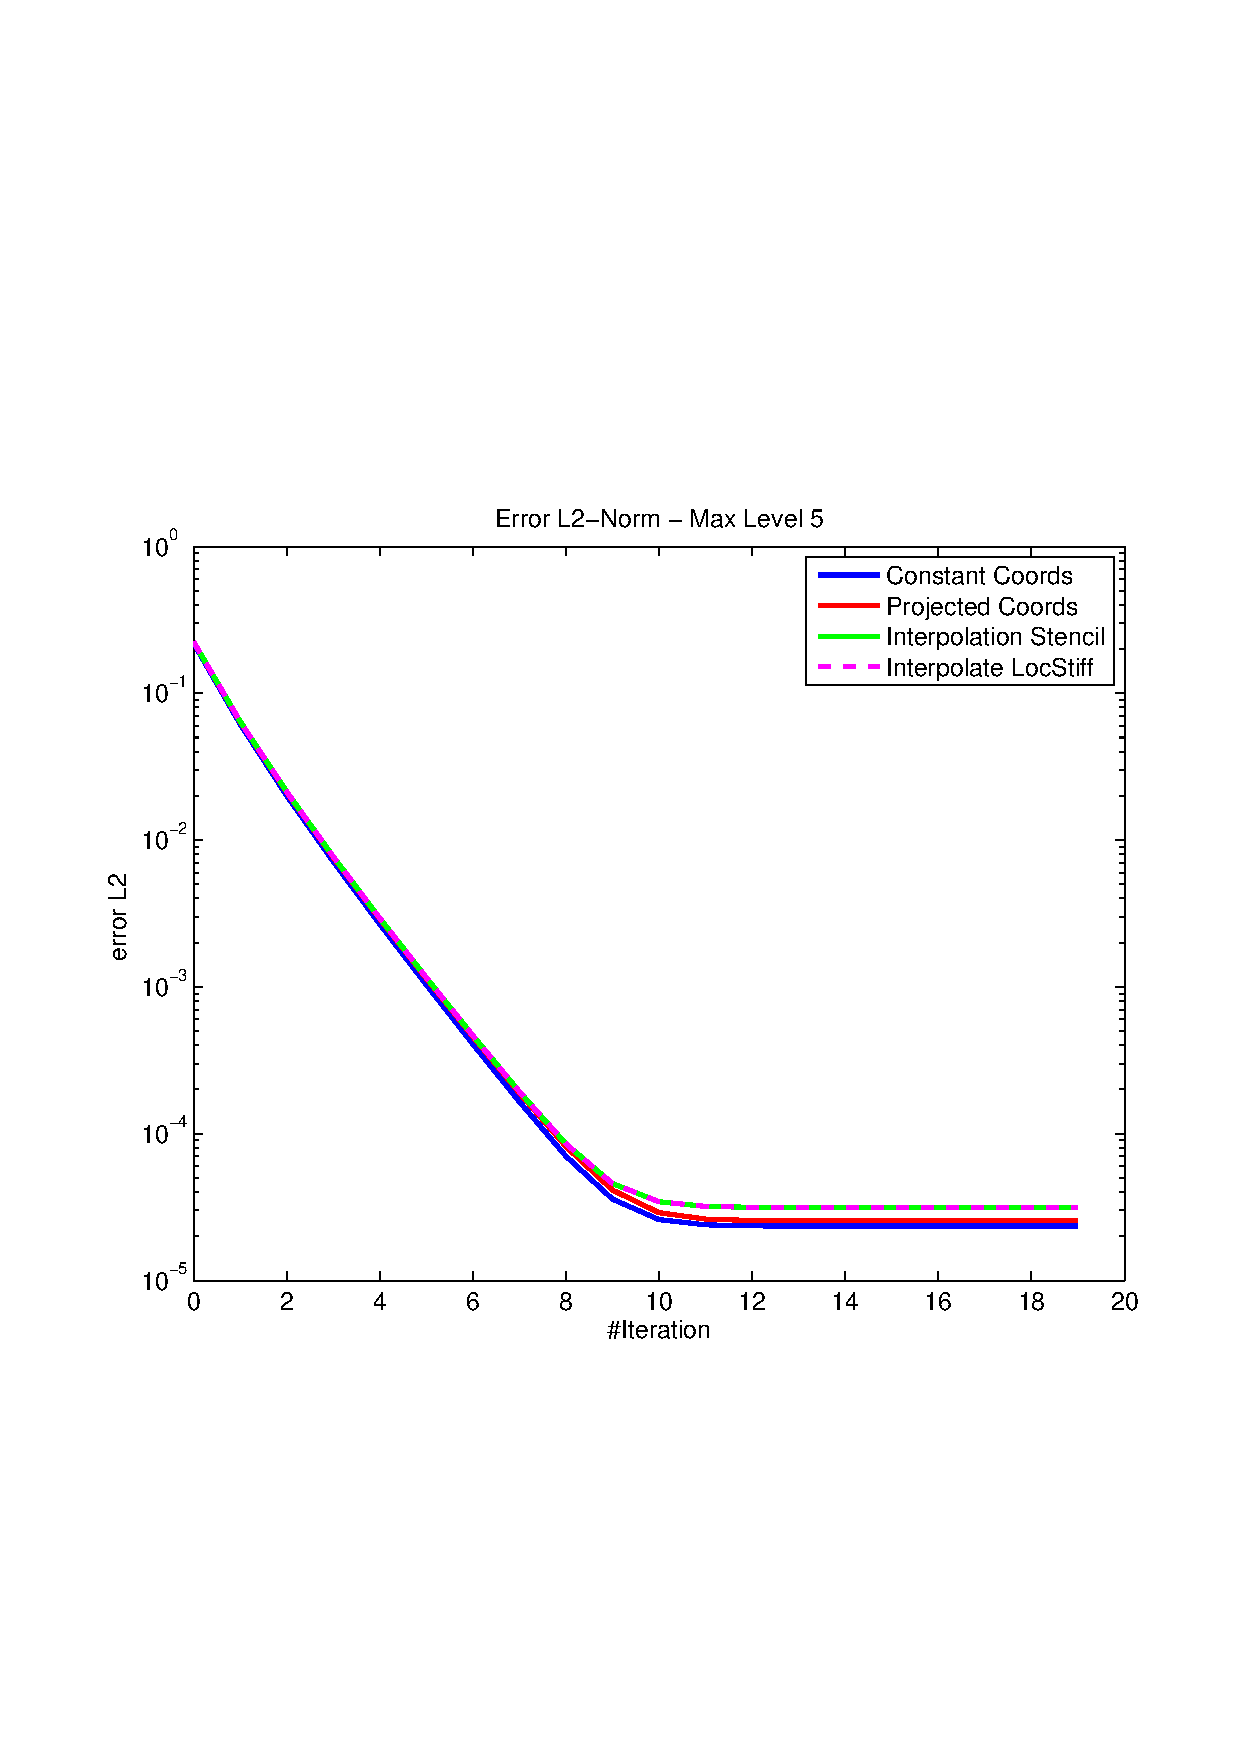
\includegraphics[width=0.98\textwidth]{spherepoisson_errorEuc_level5}\\
  max. level 5
\end{column}\hfill
\begin{column}[T]{4.3cm} 
  \centering
  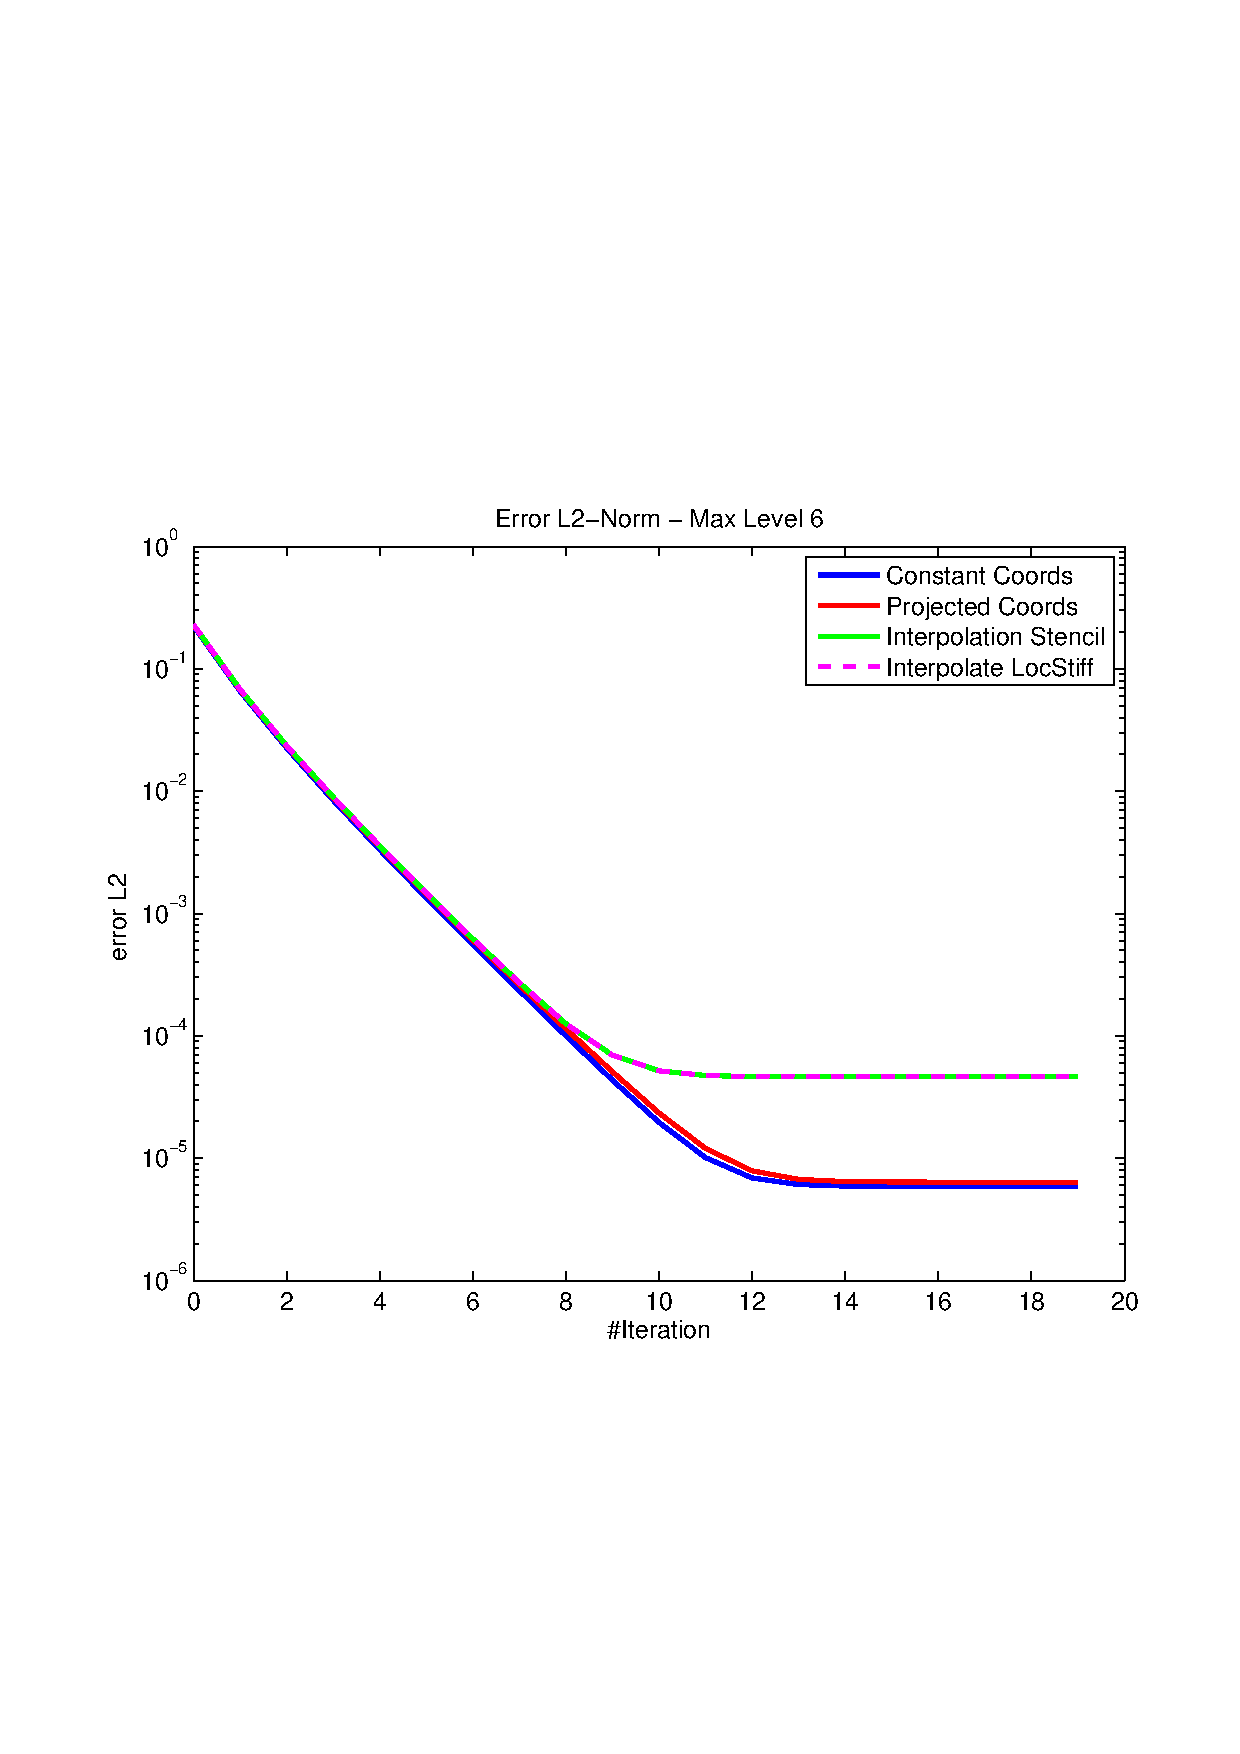
\includegraphics[width=0.98\textwidth]{spherepoisson_errorEuc_level6}\\
  max. level 6
\end{column}\hfill
\begin{column}[T]{4.3cm} 
  \centering
  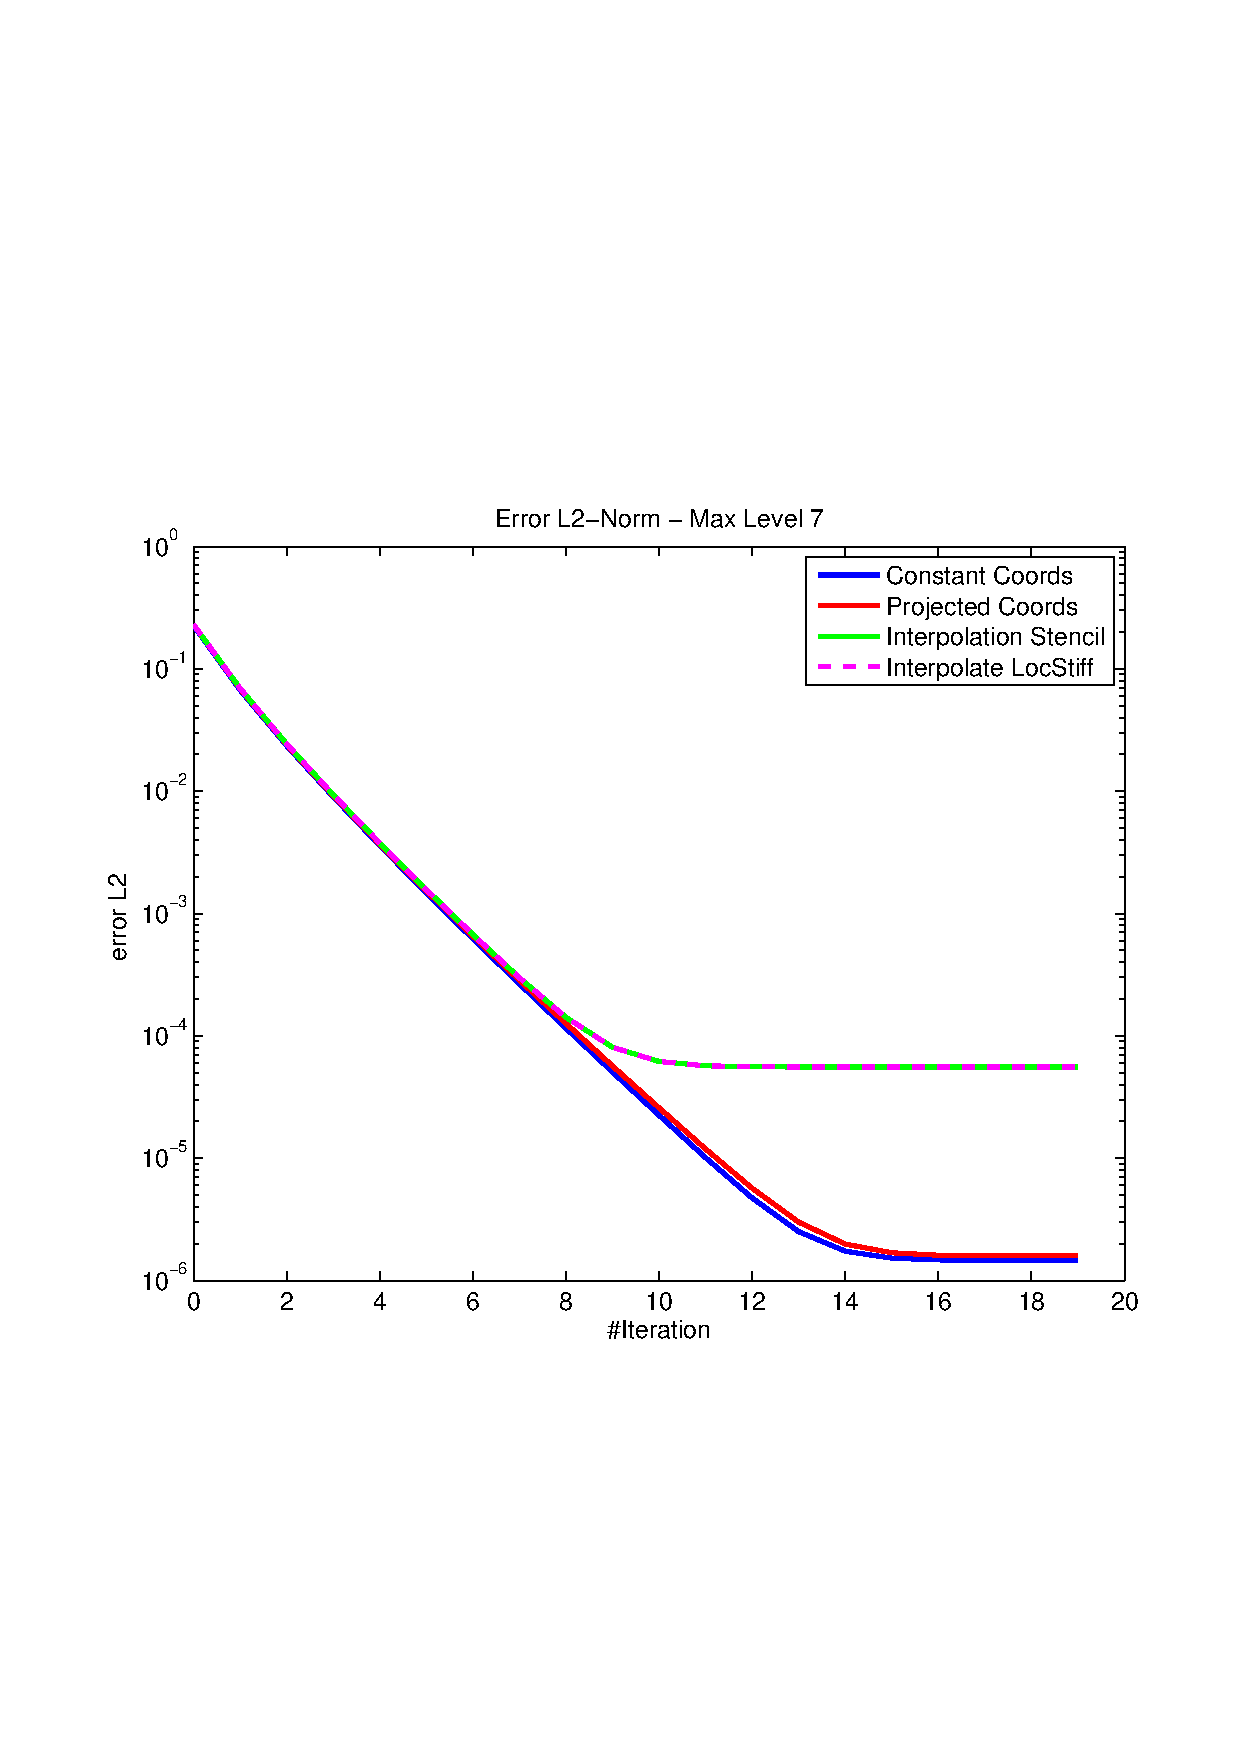
\includegraphics[width=0.98\textwidth]{spherepoisson_errorEuc_level7}\\
  max. level 7
\end{column}
\end{columns}
\vspace{0.5cm}
\centering
Comparison of discretization error for constant (blue), projected (red), interpolated
stencil (green) and interpolated local stiffness matrices (magenta).
Jobs were done on borgcube with 32 procs.
\end{frame}

%
% =============================================================================
%
\begin{frame}\frametitle{HHG results - Discretization error}

\begin{columns}[T] 
\begin{column}[T]{5.8cm} 
  \centering
  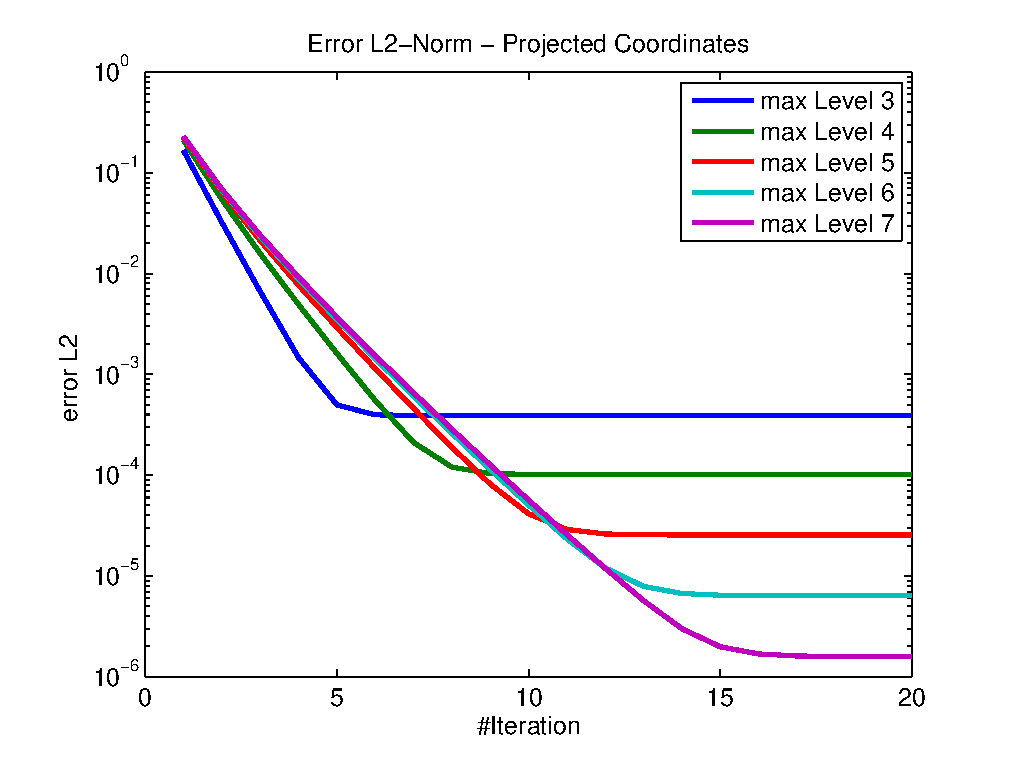
\includegraphics[width=0.98\textwidth]{spherepoisson_errorEuc_ProjCoords}\\
  projected coordinates
\end{column}\hfill
\begin{column}[T]{5.8cm} 
  \centering
  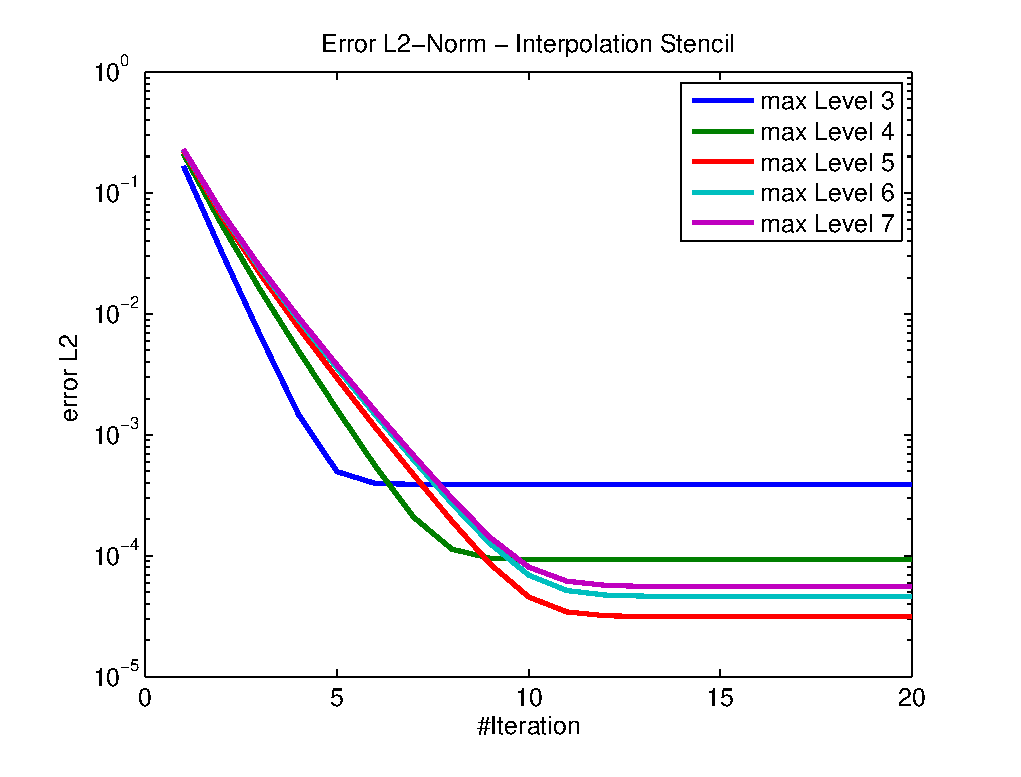
\includegraphics[width=0.98\textwidth]{spherepoisson_errorEuc_InterpolationStencil}\\
  interpolated stencils
\end{column}
\end{columns}
\vspace{0.5cm}
\centering

\end{frame}


% =============================================================================
%    Results for spherestokes
% =============================================================================
%
\section{Spherestokes}
\subsection{Spherestokes}
%
% =============================================================================
%
\begin{frame}\frametitle{HHG results - residual norm}

\begin{columns}[T] 
\begin{column}[T]{4.3cm} 
  \centering
  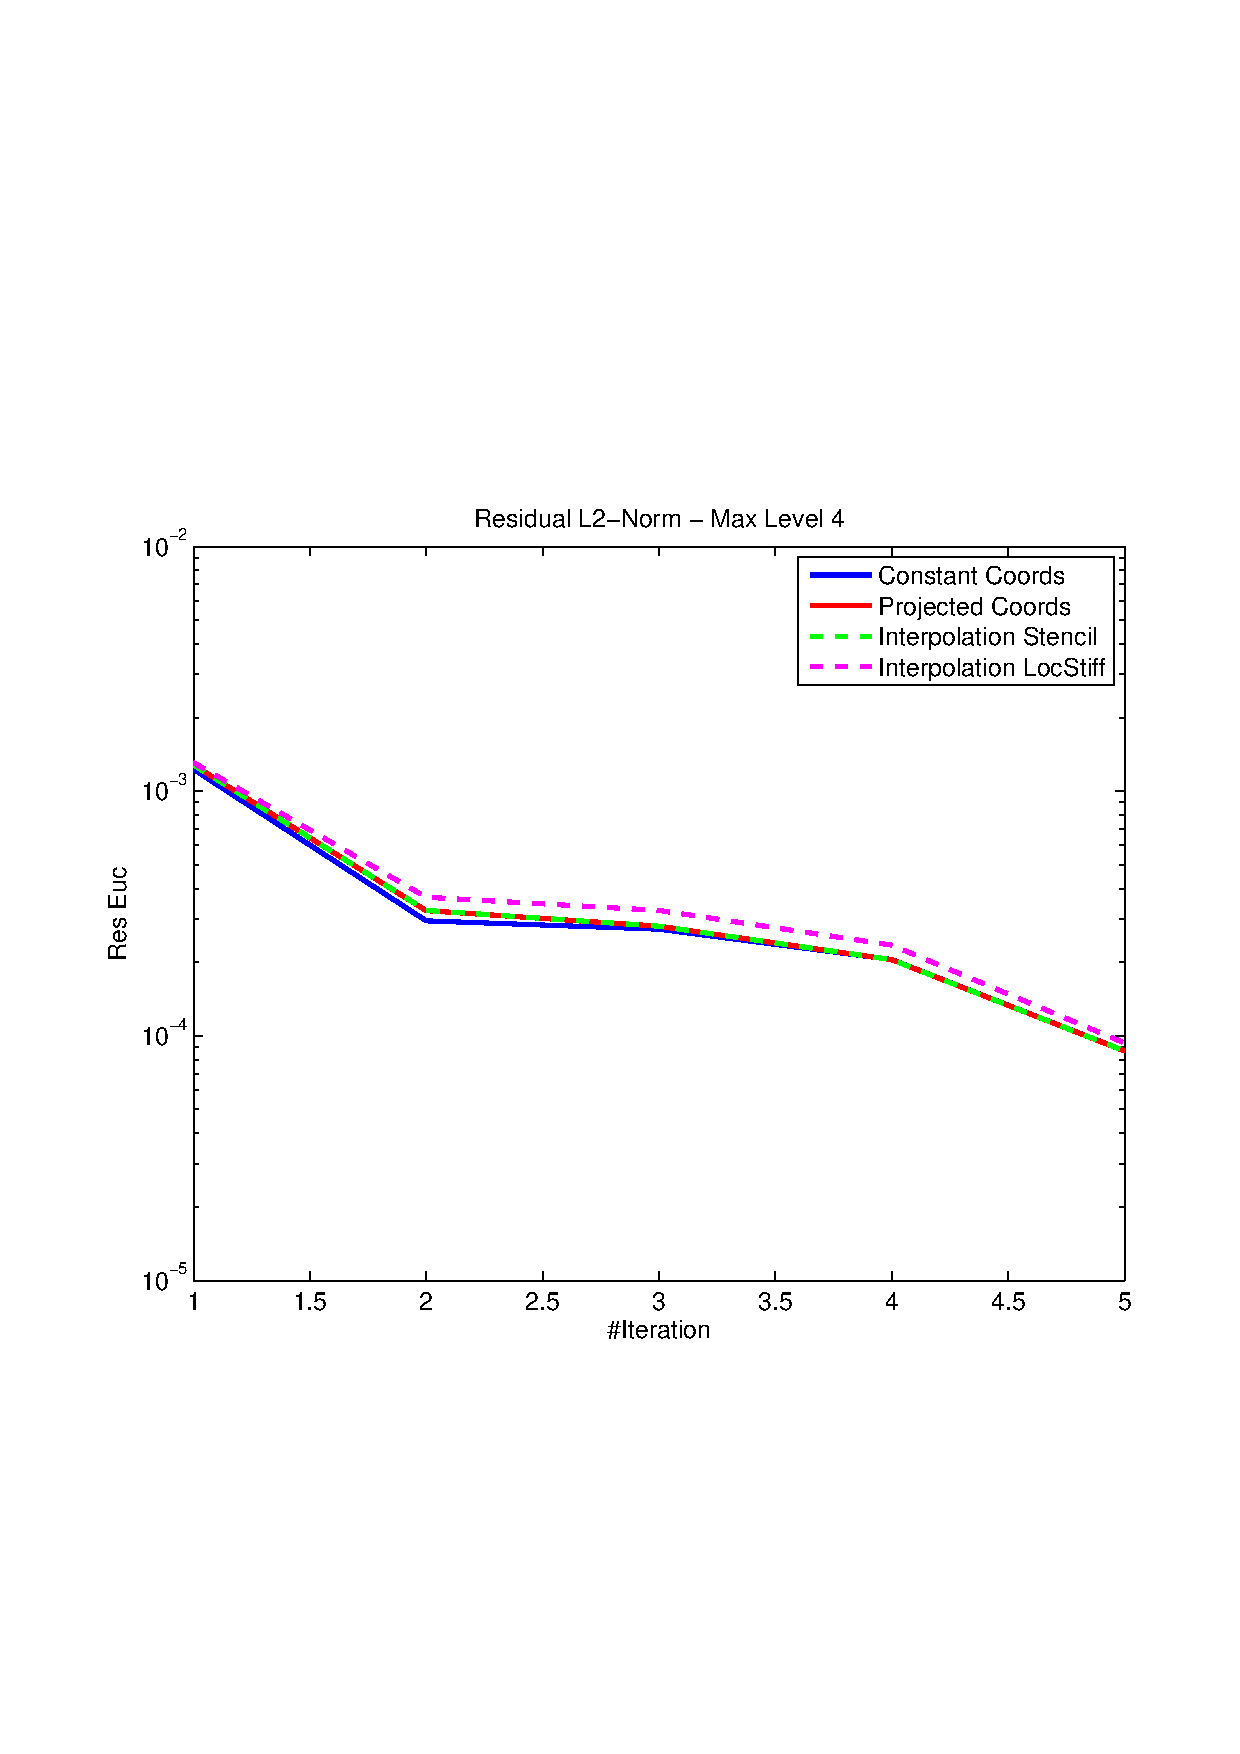
\includegraphics[width=0.98\textwidth]{spherestokes_resEuc_level4}\\
  max. level 4
\end{column}\hfill
\begin{column}[T]{4.3cm} 
  \centering
  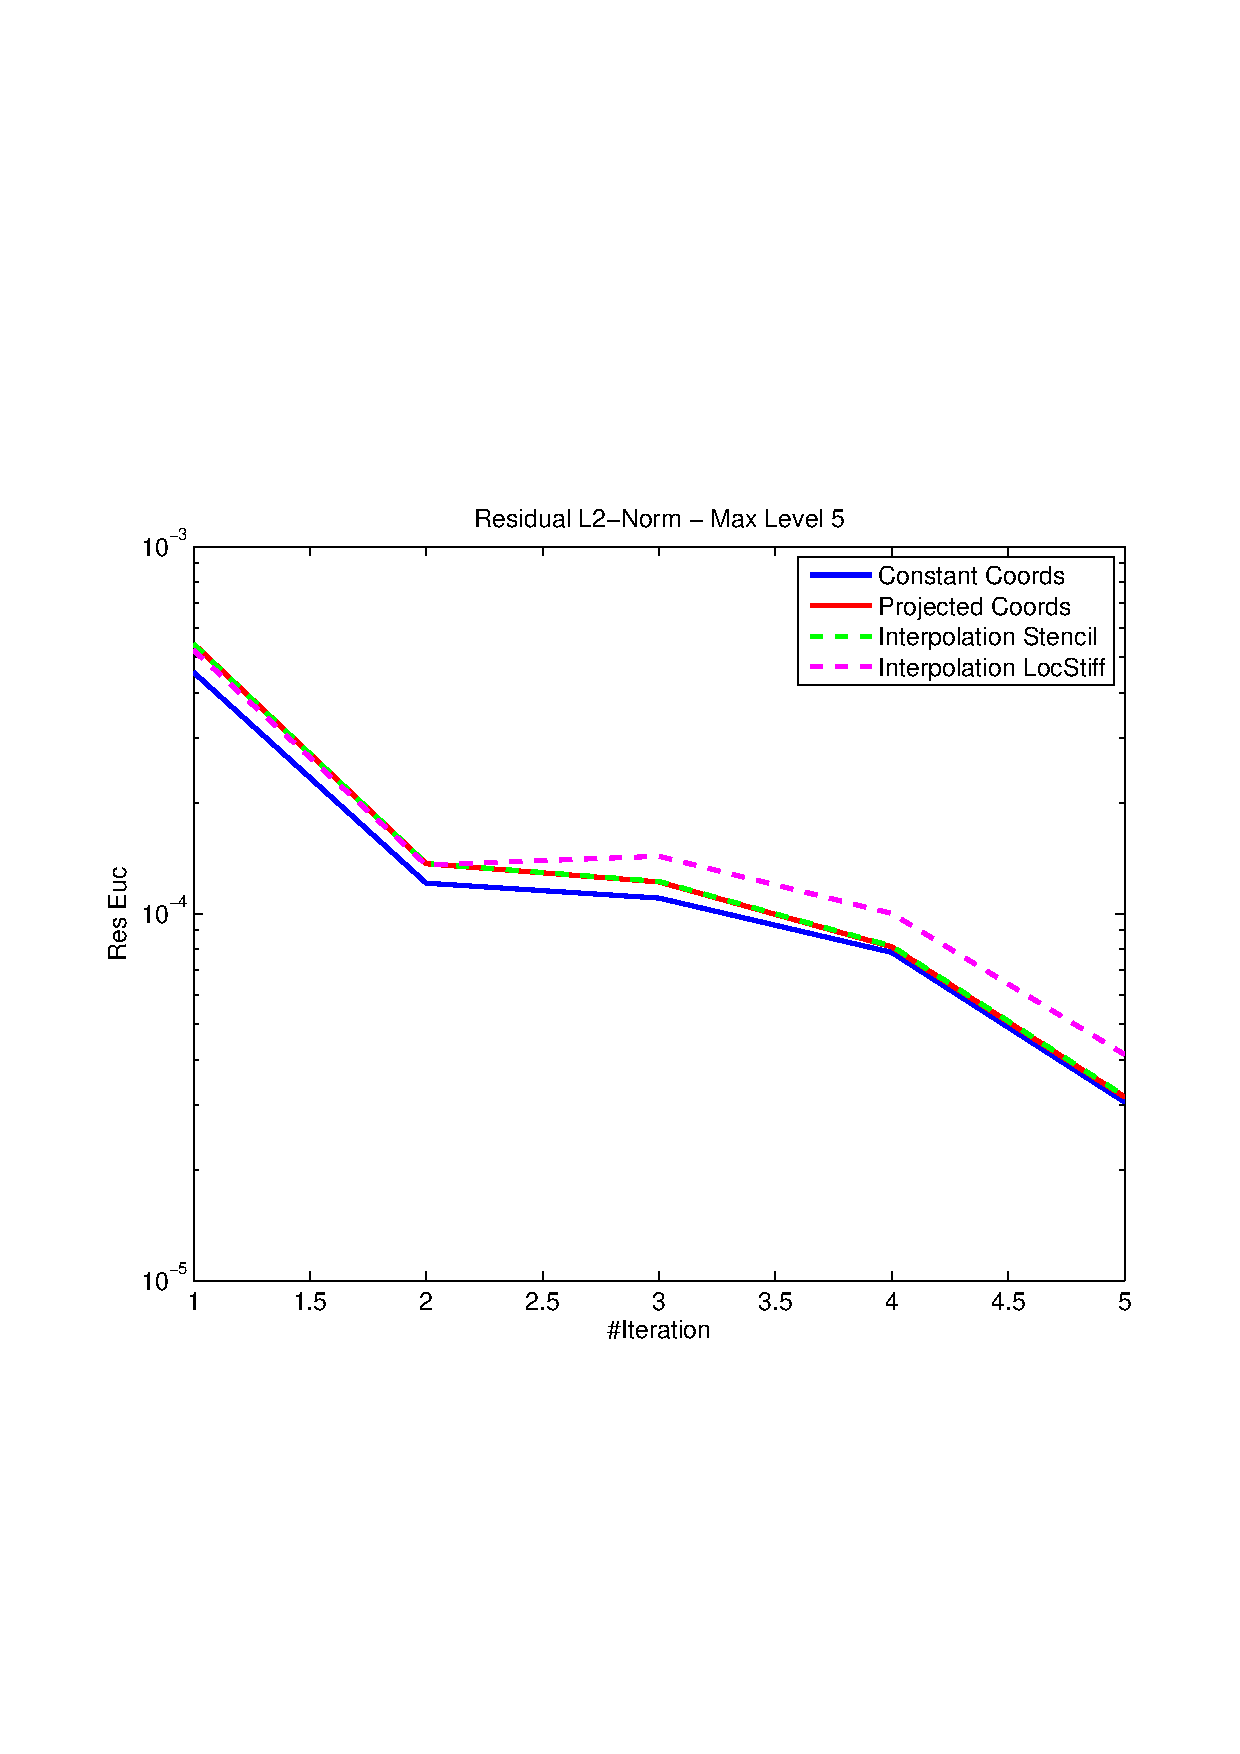
\includegraphics[width=0.98\textwidth]{spherestokes_resEuc_level5}\\
  max. level 5
\end{column}\hfill
\begin{column}[T]{4.3cm} 
  \centering
  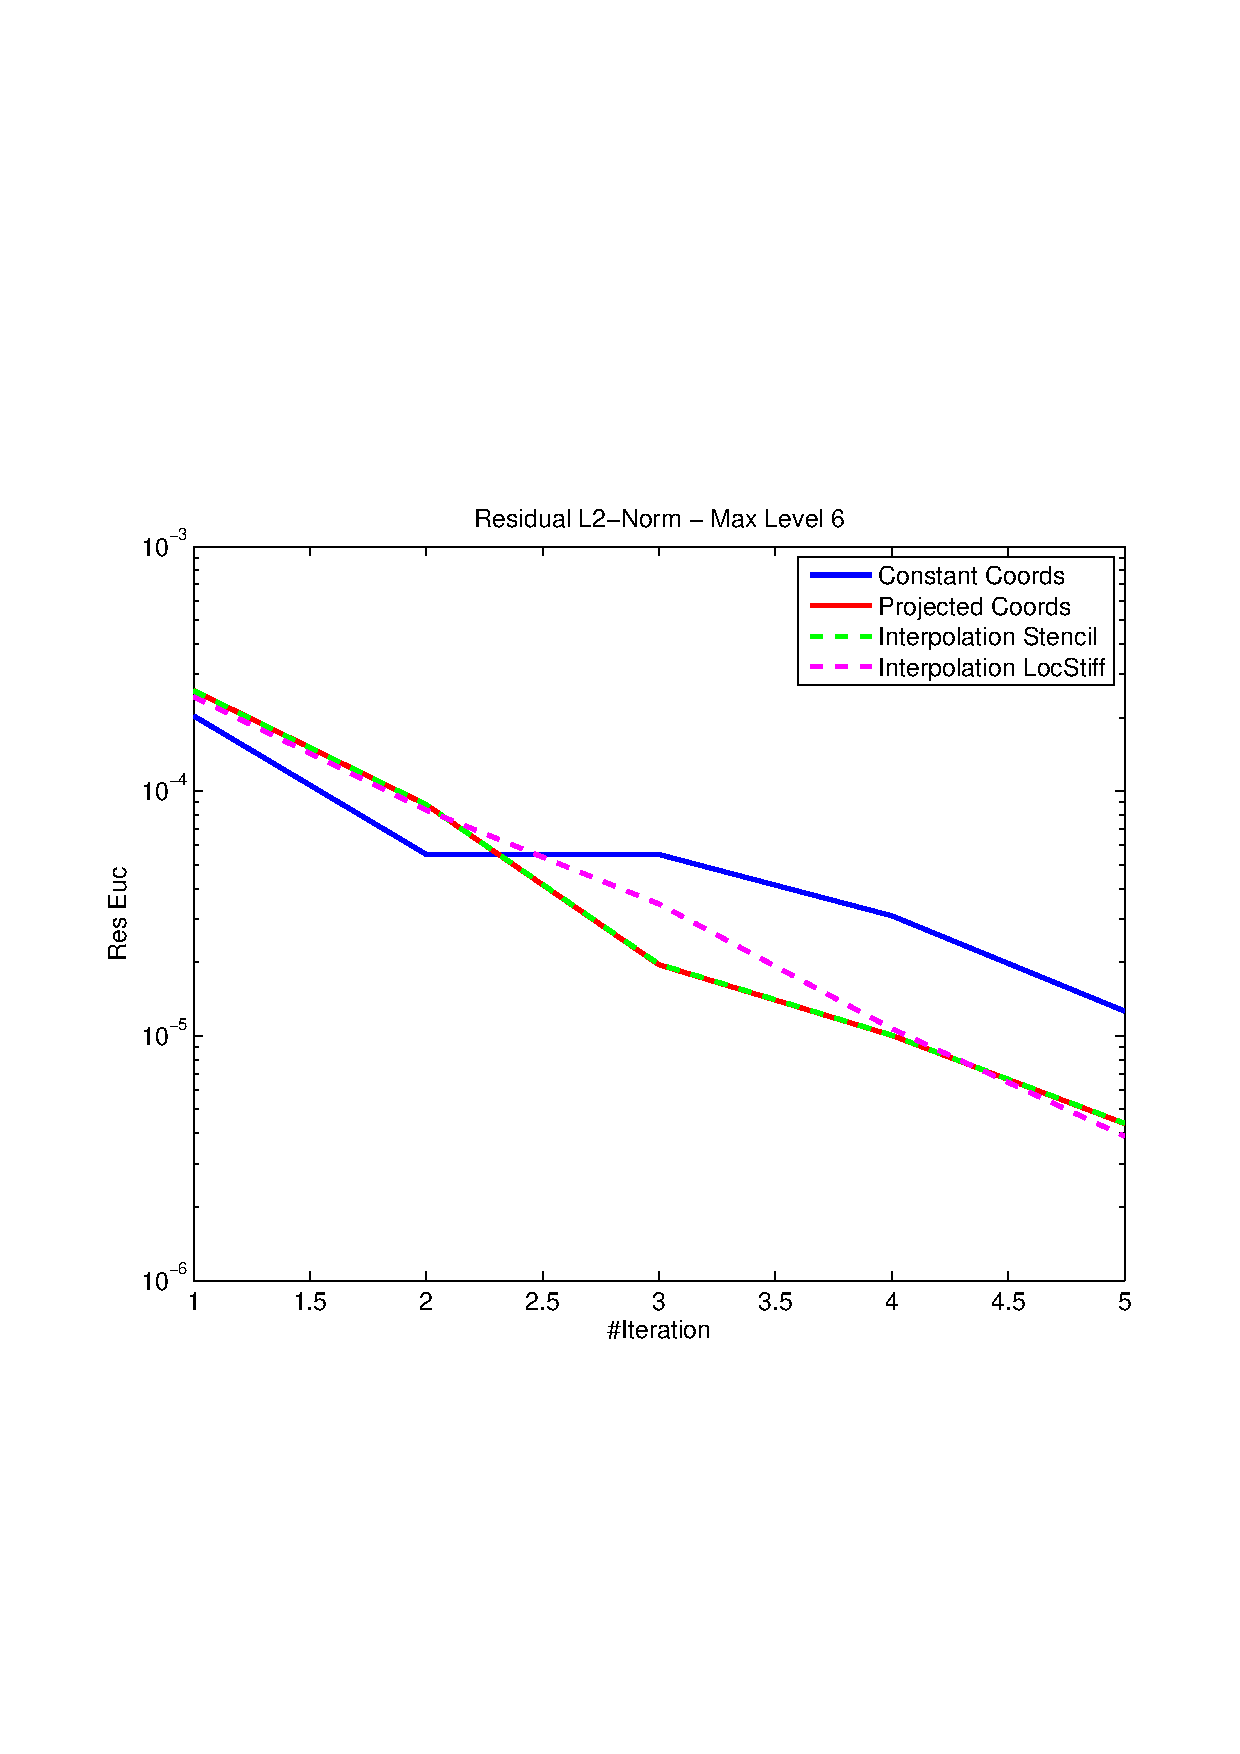
\includegraphics[width=0.98\textwidth]{spherestokes_resEuc_level6}\\
  max. level 6
\end{column}
\end{columns}
\vspace{0.5cm}
\centering
Comparison of residual for constant (blue), projected (red), interpolated
stencil (green) and interpolated local stiffness matrices (magenta)
\end{frame}
%
%
% =============================================================================
%
\begin{frame}\frametitle{HHG results - CPU time}

\begin{columns}[T] 
\begin{column}[T]{4.3cm} 
  \centering
  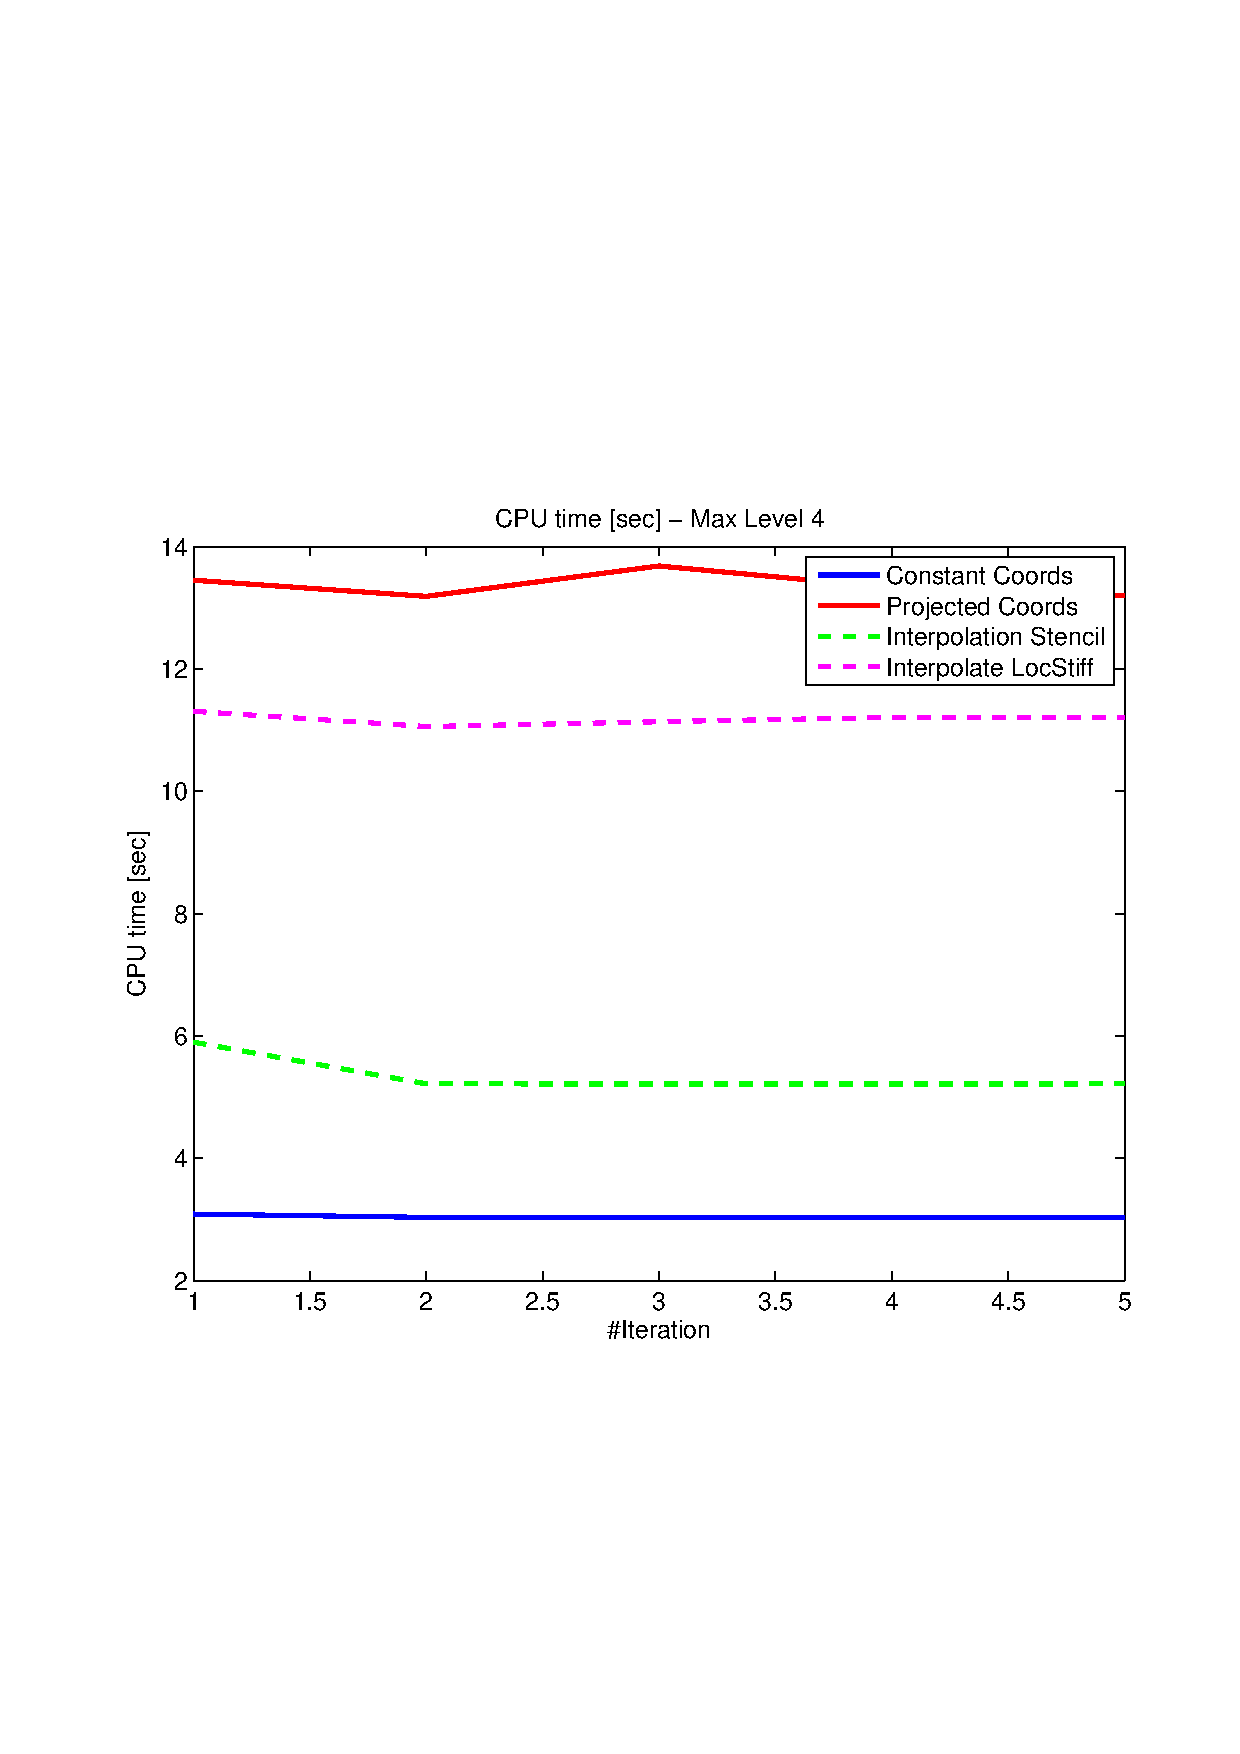
\includegraphics[width=0.98\textwidth]{spherestokes_cpuTime_level4}\\
  max. level 4
\end{column}\hfill
\begin{column}[T]{4.3cm} 
  \centering
  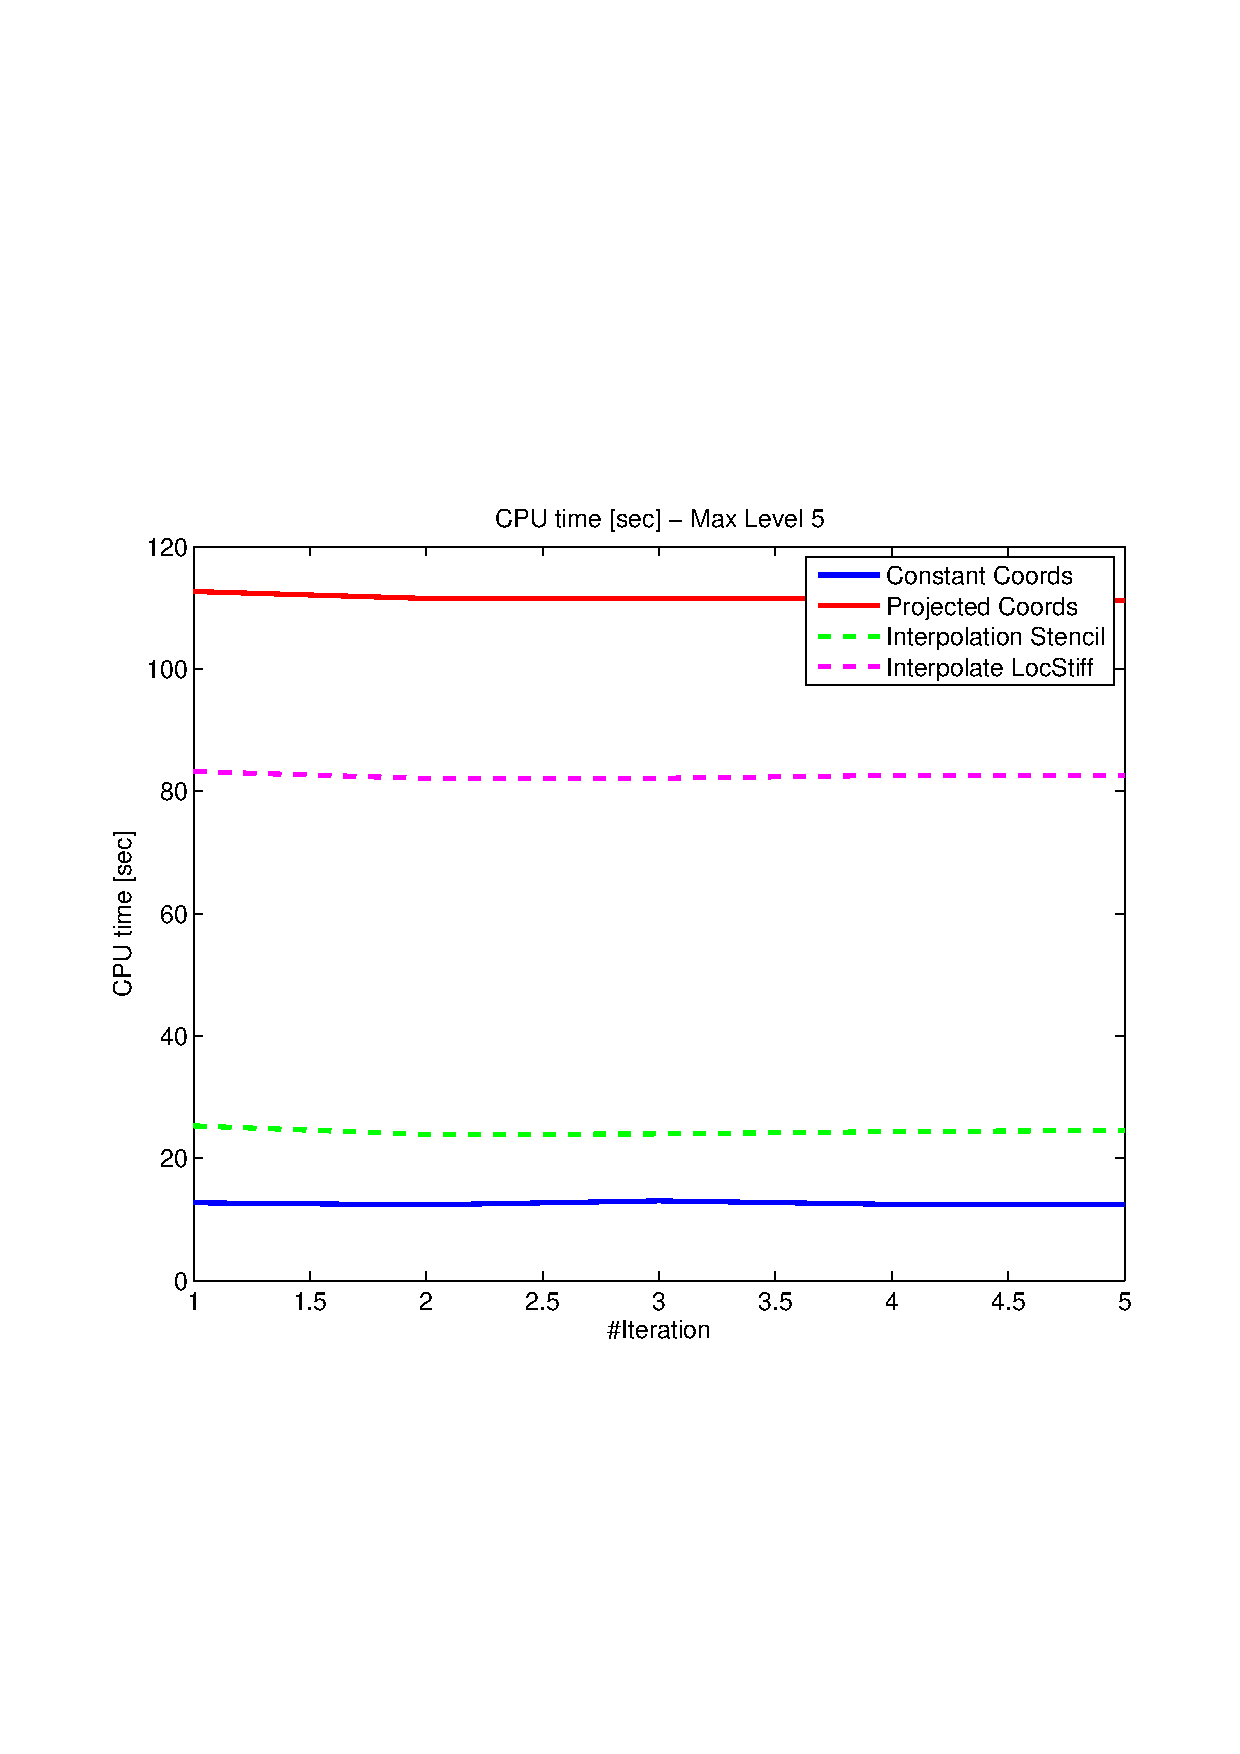
\includegraphics[width=0.98\textwidth]{spherestokes_cpuTime_level5}\\
  max. level 5
\end{column}\hfill
\begin{column}[T]{4.3cm} 
  \centering
  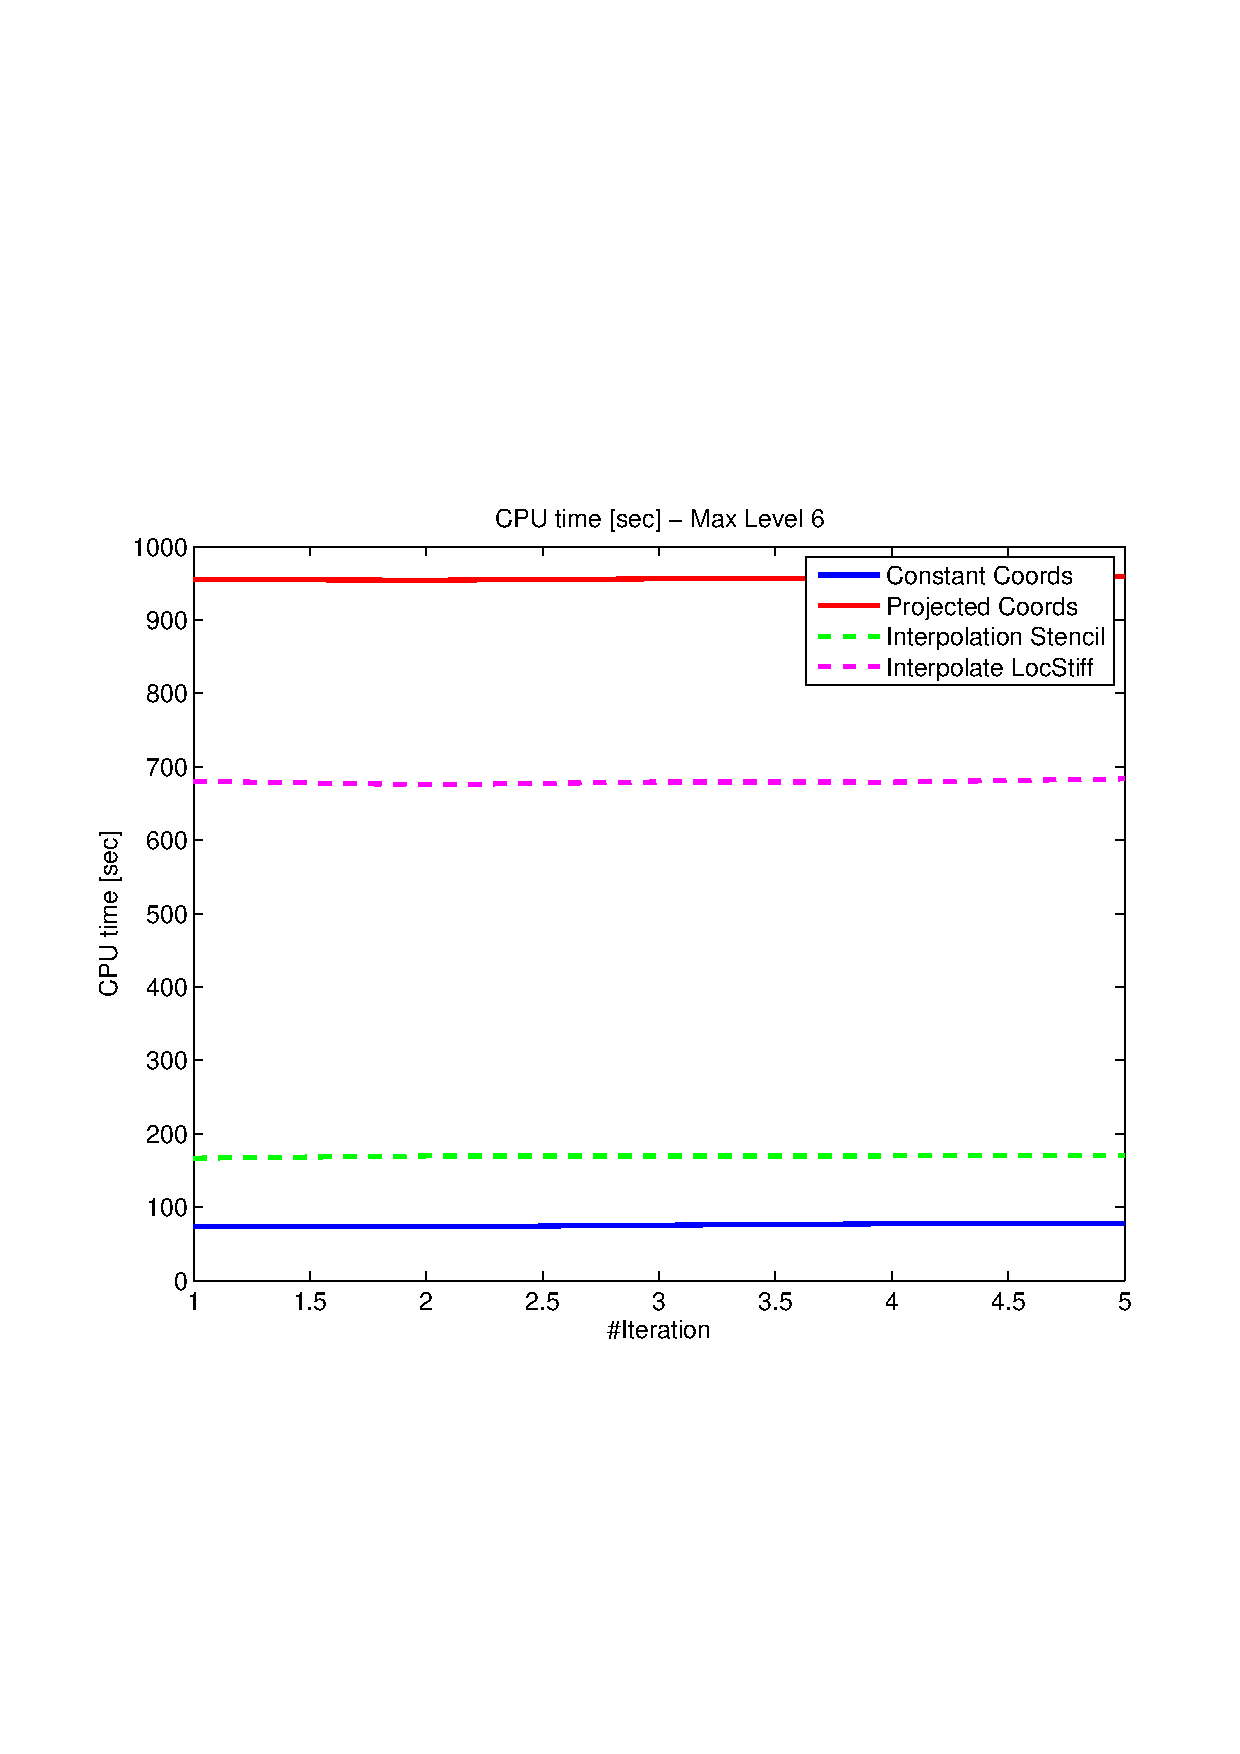
\includegraphics[width=0.98\textwidth]{spherestokes_cpuTime_level6}\\
  max. level 6
\end{column}
\end{columns}
\vspace{0.5cm}
\centering
Comparison of CPU time [sec] for constant (blue), projected (red), interpolated
stencil (green) and interpolated local stiffness matrices (magenta).
Jobs were done on borgcube with 32 procs.
\end{frame}

%
% =============================================================================
%
\begin{frame}\frametitle{HHG results - Discretization error}

\begin{columns}[T] 
\begin{column}[T]{4.3cm} 
  \centering
  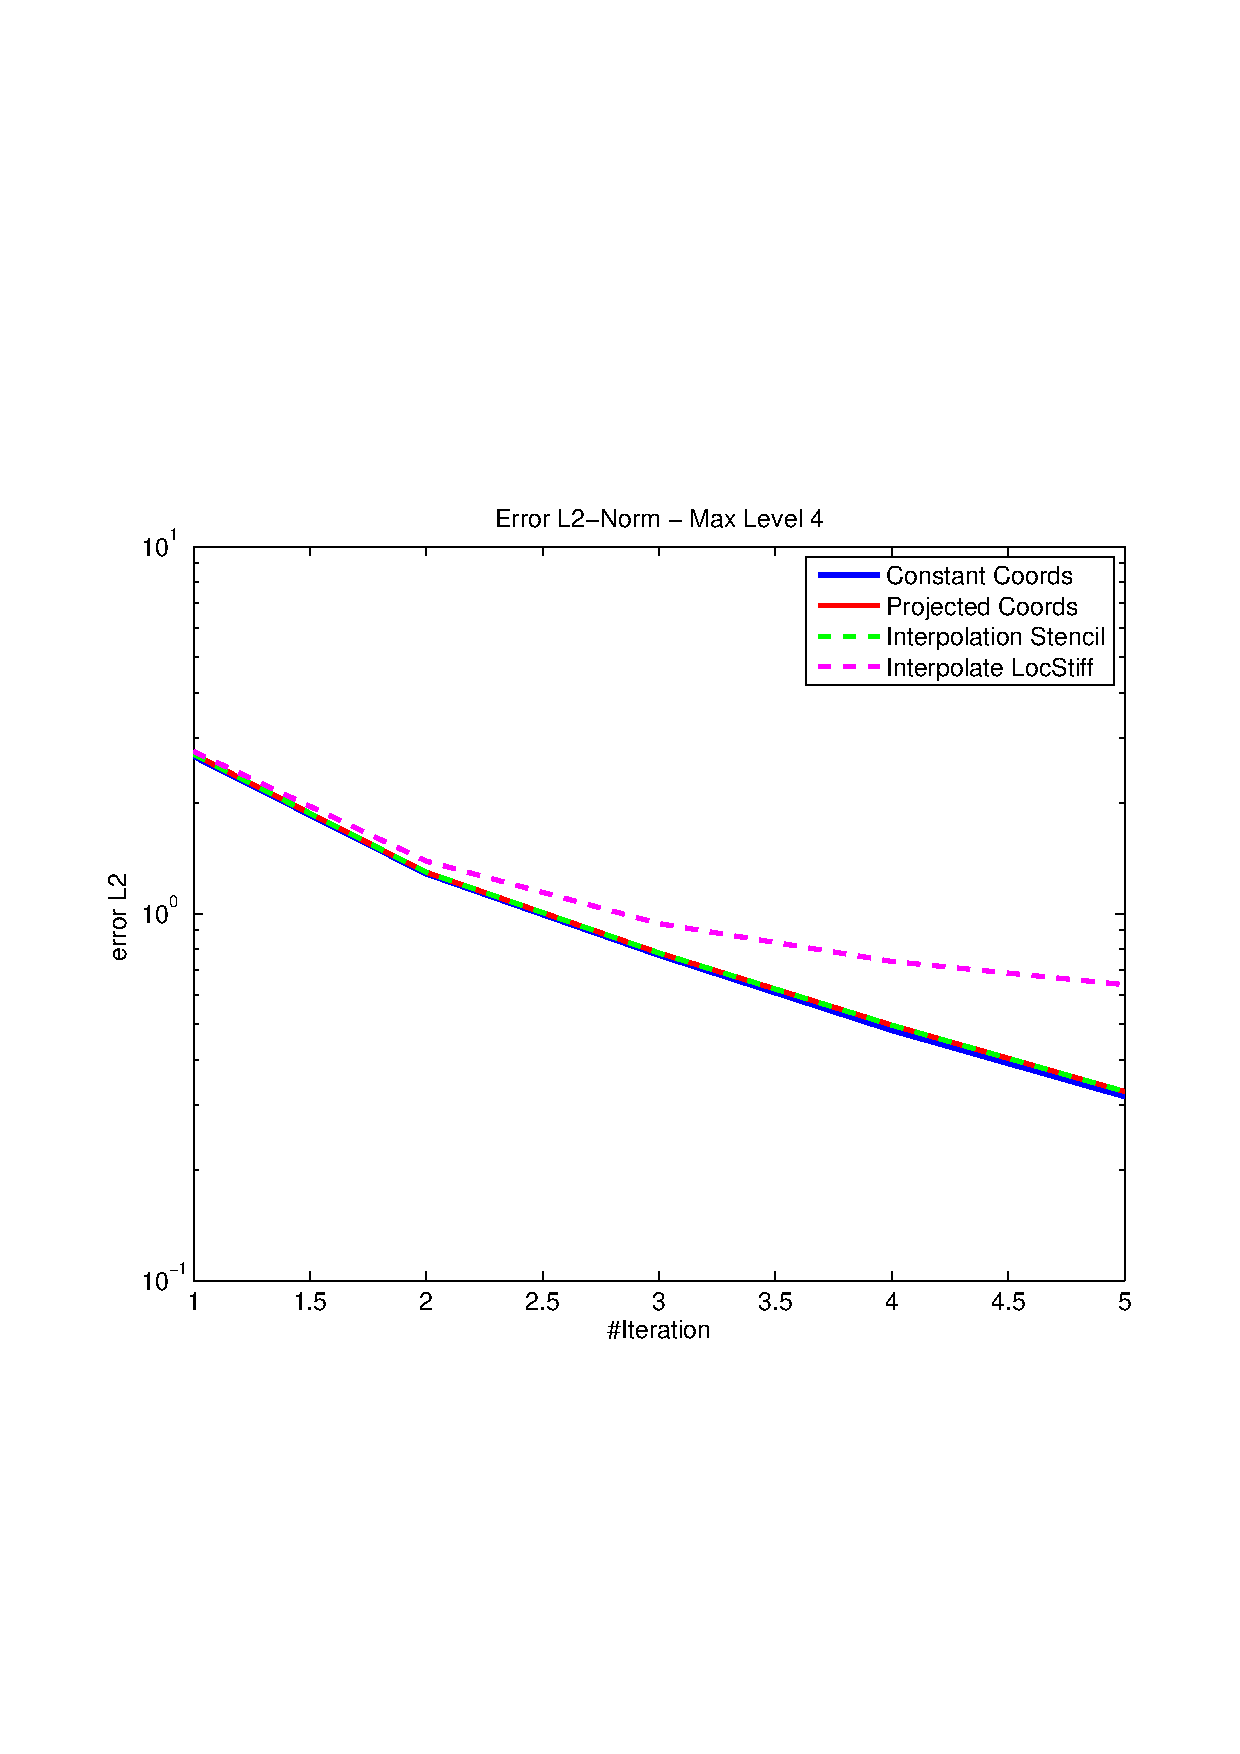
\includegraphics[width=0.98\textwidth]{spherestokes_errorEuc_level4}\\
  max. level 4
\end{column}\hfill
\begin{column}[T]{4.3cm} 
  \centering
  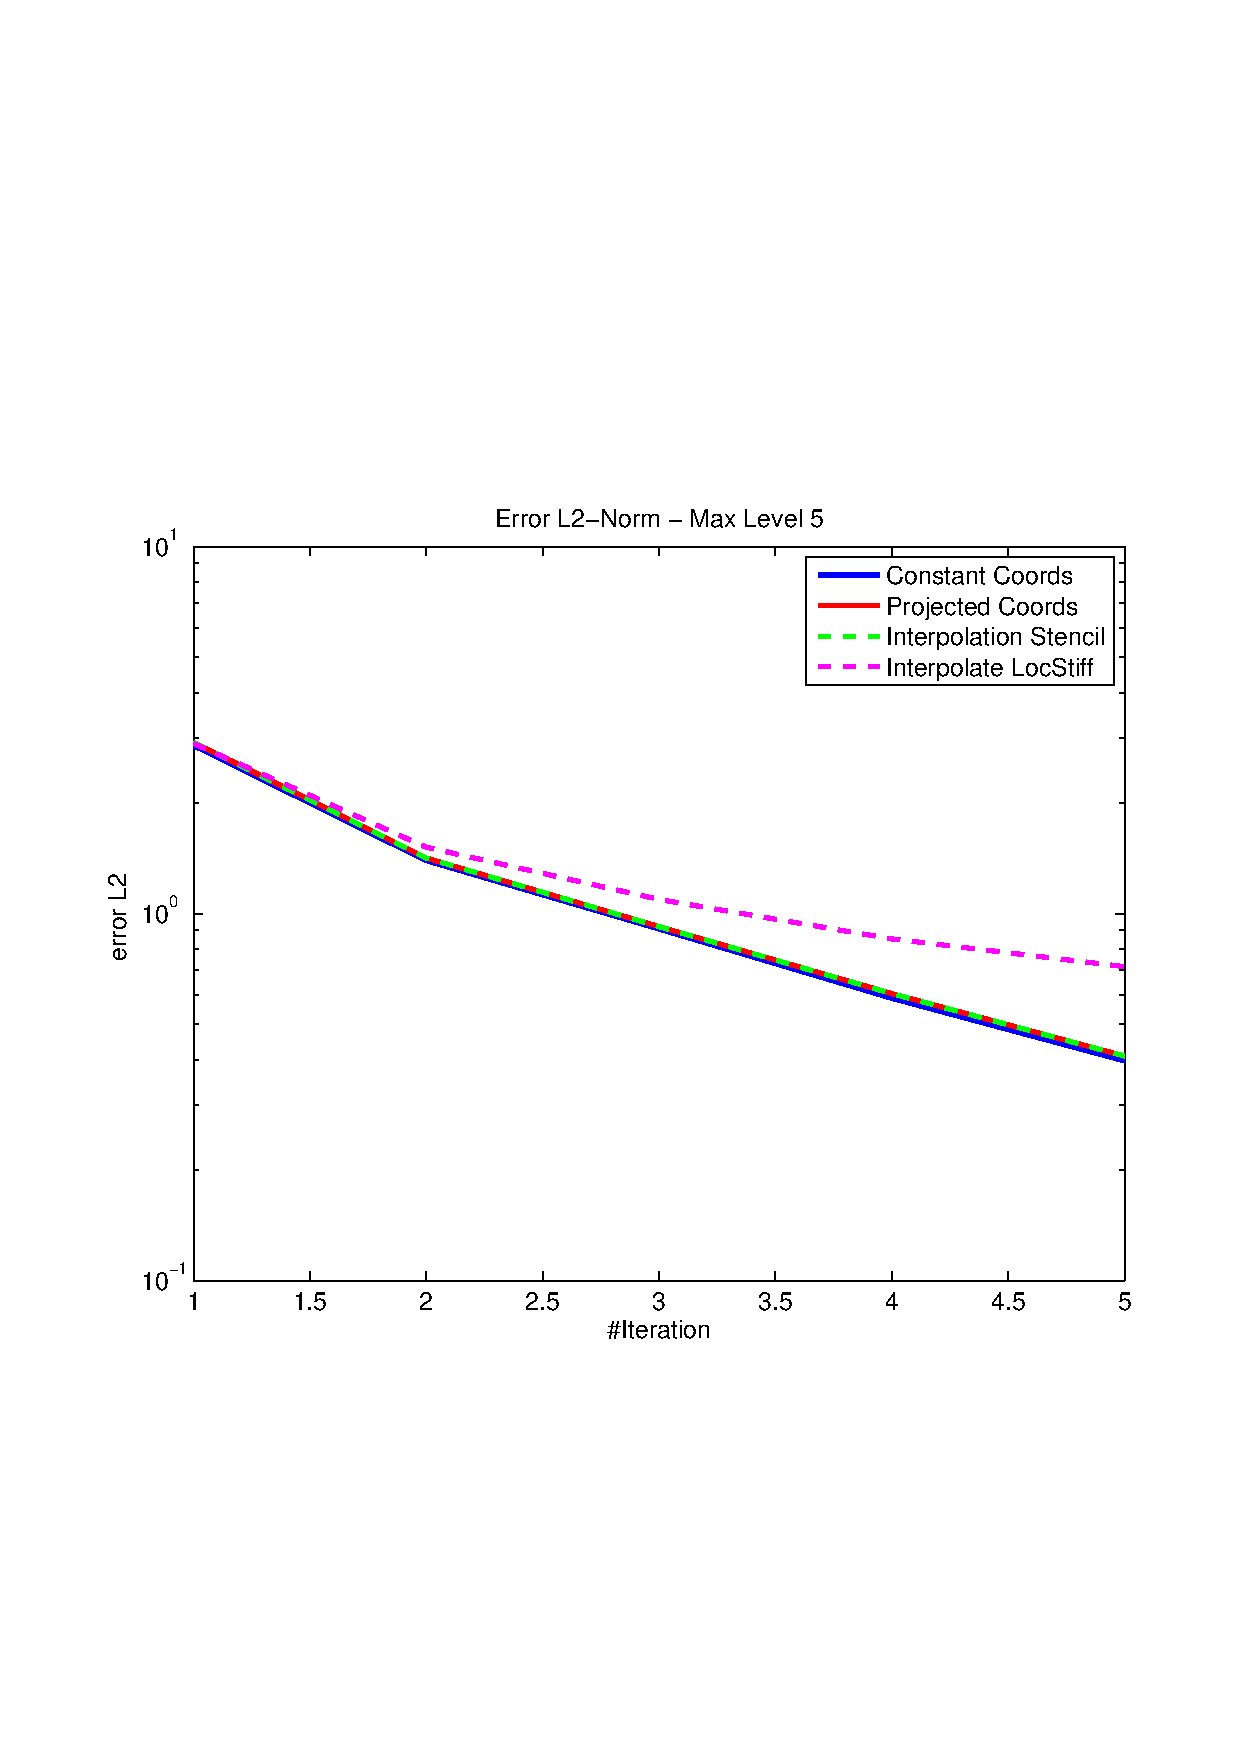
\includegraphics[width=0.98\textwidth]{spherestokes_errorEuc_level5}\\
  max. level 5
\end{column}\hfill
\begin{column}[T]{4.3cm} 
  \centering
  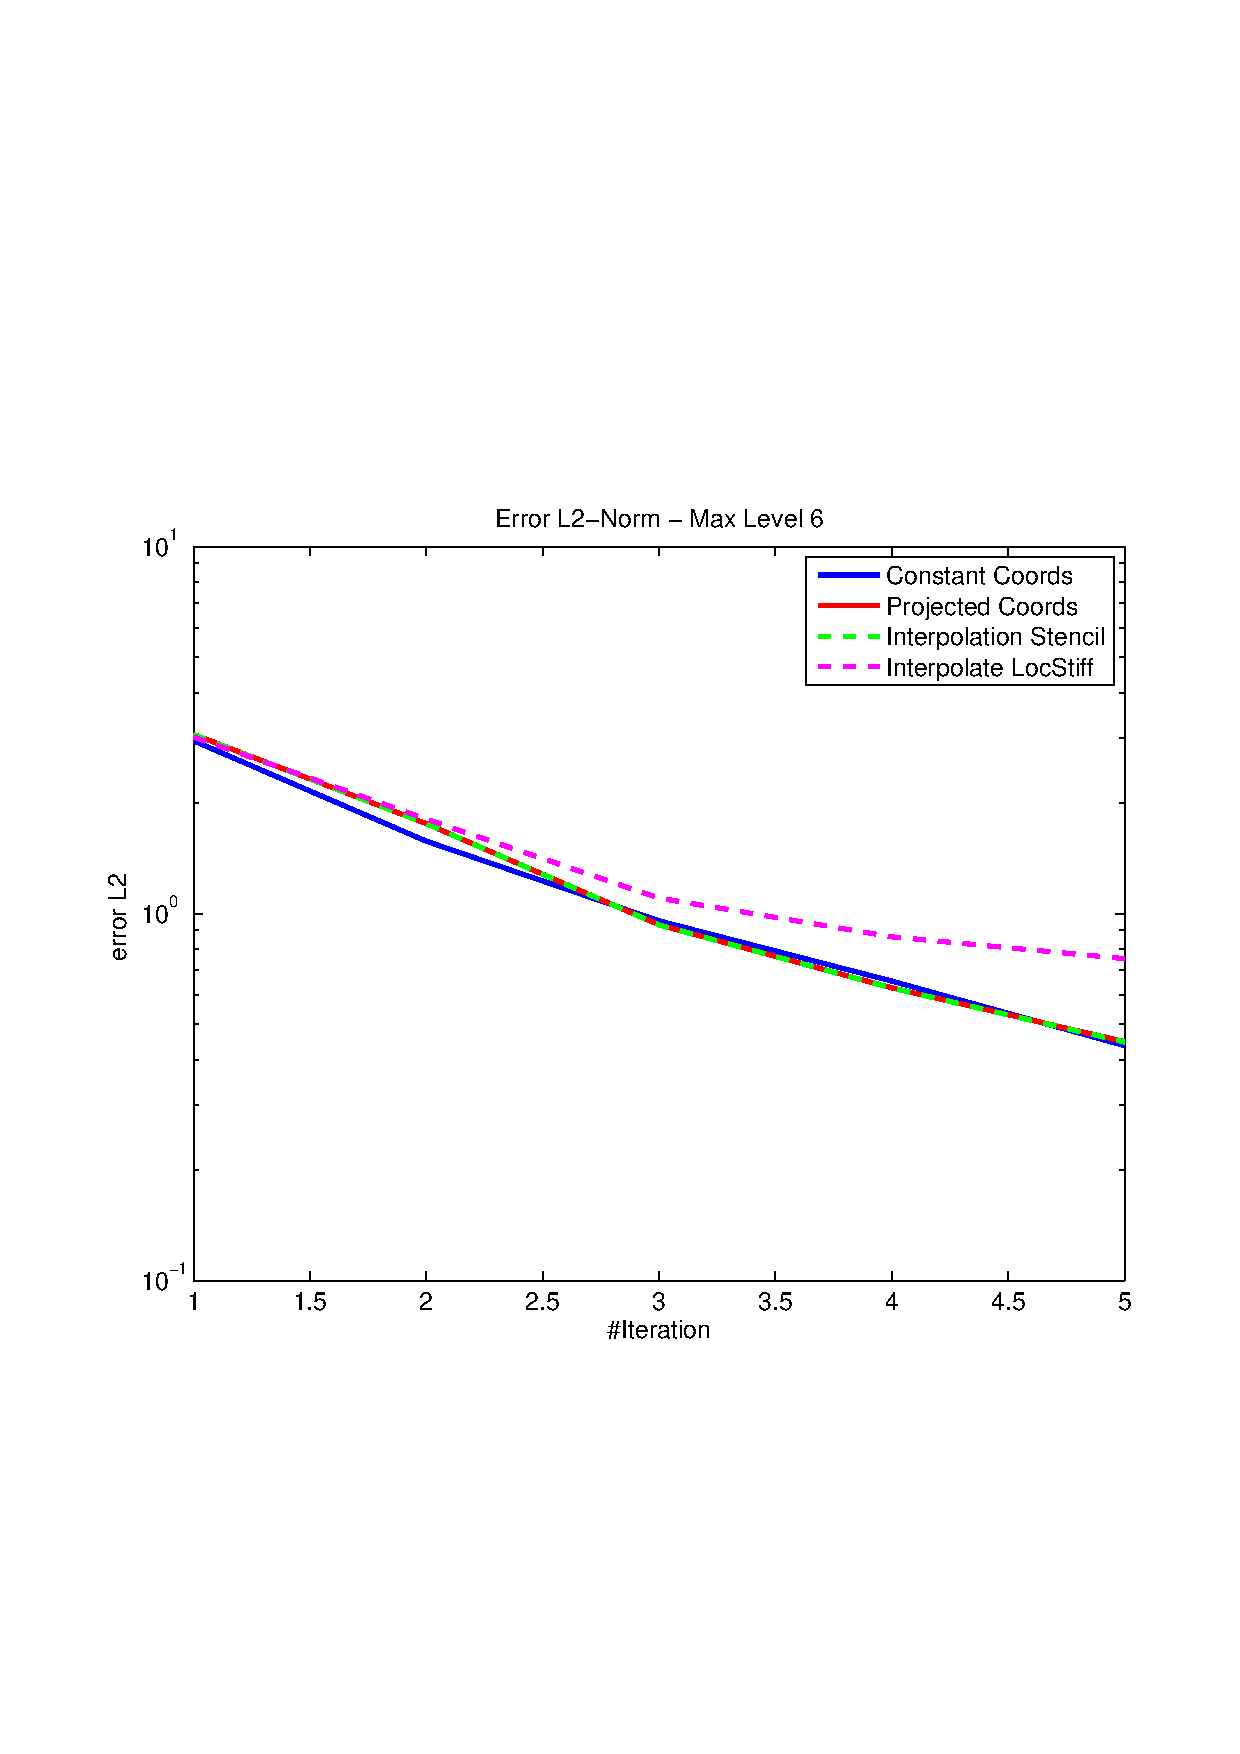
\includegraphics[width=0.98\textwidth]{spherestokes_errorEuc_level6}\\
  max. level 6
\end{column}
\end{columns}
\vspace{0.5cm}
\centering
Comparison of discretization error for constant (blue), projected (red), interpolated
stencil (green) and interpolated local stiffness matrices (magenta).
Jobs were done on borgcube with 32 procs.
\end{frame}

% =============================================================================
%    Outlook
% =============================================================================
%
\section{Outlook}
\subsection{Outlook}
%
\begin{frame}\frametitle{Outlook}
%
todo...
%
\end{frame}
%
% =============================================================================
\end{document}
% =============================================================================
% EOF
% =============================================================================
